% !TeX program = xelatex
% !TeX encoding = UTF-8
% Presentazione revisionata: Prisma · Classificazione e validazione
% Basata sul materiale originale fornito dall'autore e sul template M01_Pensare_con_i_dati.tex
% Compilazione: xelatex -interaction=nonstopmode M16_Prisma.tex (due passaggi)
% Diagrammi TikZ e figure statistiche vettoriali; sorgenti R e dati inclusi.
% 62 slide. Materiali del corso e impaginazione della serie planetaria.
\RequirePackage{fix-cm}
\documentclass[12pt,aspectratio=1610]{beamer}
\geometry{paperwidth=20cm,paperheight=12.5cm}
\usepackage[italian,provide=*]{babel}
\usepackage{fontspec,adjustbox,tabularx}
\IfFontExistsTF{NimbusSans-Regular.otf}{
\setsansfont{NimbusSans-Regular.otf}[BoldFont=NimbusSans-Bold.otf,ItalicFont=NimbusSans-Italic.otf,BoldItalicFont=NimbusSans-BoldItalic.otf]
\setmainfont{NimbusSans-Regular.otf}[BoldFont=NimbusSans-Bold.otf,ItalicFont=NimbusSans-Italic.otf,BoldItalicFont=NimbusSans-BoldItalic.otf]
}{
\setsansfont{TeX Gyre Heros}
\setmainfont{TeX Gyre Heros}
}
\IfFontExistsTF{DejaVu Sans Mono}{
\setmonofont{DejaVu Sans Mono}[Scale=.88]
}{\setmonofont{Latin Modern Mono}[Scale=.88]}
\usefonttheme{professionalfonts}
\usepackage{amsmath,amssymb,booktabs,array,graphicx,tikz,bookmark}
\usetikzlibrary{calc,positioning,arrows.meta}
\graphicspath{{Figure/}}
\definecolor{Paper}{HTML}{F8F6F1}
\definecolor{Ink}{HTML}{253344}
\definecolor{Navy}{HTML}{15283E}
\definecolor{Quantum}{HTML}{5146A5}
\definecolor{Classical}{HTML}{087C74}
\definecolor{Muted}{HTML}{657180}
\definecolor{Rule}{HTML}{D6DAD9}
\definecolor{Night}{HTML}{112236}
\definecolor{Lilac}{HTML}{ABB5FF}
\definecolor{Mint}{HTML}{72D8C8}
\setbeamercolor{background canvas}{bg=Paper}
\setbeamercolor{normal text}{fg=Ink}
\setbeamertemplate{navigation symbols}{}
\setbeamertemplate{headline}{}
\setbeamertemplate{footline}{}
\setbeamersize{text margin left=0pt,text margin right=0pt}
\hypersetup{colorlinks=true,linkcolor=Classical,urlcolor=Classical,pdfpagemode=UseOutlines,pdfstartview=Fit,
 pdftitle={Prisma · Classificazione e validazione},pdfauthor={GeoStat Lab · materiali di Marzio De Corato},
 pdfsubject={GeoStat Lab · M16}}
\bookmarksetup{open,openlevel=0,depth=2}
\newsavebox{\BodyBox}
\newsavebox{\SideBox}
\newsavebox{\RecallBox}
\newsavebox{\TitleBox}
\newcommand{\MeasureBox}[2]{\typeout{REVIEWBOX:#1:\the\wd#2:\the\ht#2:\the\dp#2}}

% Revisione completa: diagrammi TikZ, formalismo e box R.
\usepackage[most]{tcolorbox}
\usepackage{listings}
\usetikzlibrary{fit,backgrounds,matrix,decorations.pathreplacing}
\definecolor{GeoA}{HTML}{1D7890}
\definecolor{GeoB}{HTML}{C57E42}
\definecolor{GeoC}{HTML}{7363AA}
\definecolor{GeoTint}{HTML}{F0F4F3}
\lstdefinestyle{GeoR}{language=R,basicstyle=\ttfamily\fontsize{9.2}{12.2}\selectfont,
 keywordstyle=\color{Quantum}\bfseries,commentstyle=\color{Classical},stringstyle=\color{GeoB},
 numbers=left,numberstyle=\tiny\color{Muted},numbersep=4pt,showstringspaces=false,
 columns=fullflexible,keepspaces=true,breaklines=true,xleftmargin=1.15em,
 frame=none,aboveskip=0pt,belowskip=0pt,tabsize=2}
\newsavebox{\PilotLeftBox}
\newsavebox{\PilotRightBox}
\newcommand{\PLabel}[1]{\par{\color{Classical}\bfseries\fontsize{9}{11}\selectfont\MakeUppercase{#1}}\par\vspace{1.8mm}}
\newcommand{\PBody}[1]{\par{\fontsize{11.3}{14.8}\selectfont #1\par}}
\newcommand{\PSmall}[1]{\par{\fontsize{9.8}{13.1}\selectfont #1\par}}
\newcommand{\PCode}[2]{%
\begin{tcolorbox}[enhanced,arc=1.8mm,boxrule=.65pt,
  colback=white,colframe=Classical!75!Navy,colbacktitle=Navy,
  coltitle=white,fonttitle=\bfseries\fontsize{9.6}{12}\selectfont,
  title={#1},left=1.7mm,right=1.3mm,top=1.5mm,bottom=1.3mm,
  before skip=1mm,after skip=1mm]
\lstinputlisting[style=GeoR]{Codice/#2}
\end{tcolorbox}}
\newcommand{\PInfo}[1]{%
\begin{tcolorbox}[enhanced,arc=1.6mm,boxrule=.55pt,colback=GeoTint,
 colframe=Rule!80!Classical,left=2.3mm,right=2.3mm,top=2mm,bottom=2mm,
 before skip=1mm,after skip=1mm]
\PSmall{#1}\end{tcolorbox}}
\tikzset{
 pFlow/.style={draw=Classical!45,fill=white,rounded corners=2mm,
  line width=.7pt,align=center,minimum height=1.1cm,font=\sffamily\fontsize{10}{12}\selectfont},
 pEdge/.style={-{Latex[length=2.3mm]},draw=Classical,line width=.95pt},
 pGroup/.style={draw=Rule,fill=white,rounded corners=2mm,line width=.65pt},
 pDotA/.style={circle,fill=GeoA,inner sep=1.25pt},
 pDotB/.style={circle,fill=GeoB,inner sep=1.25pt},
 pDotC/.style={circle,fill=GeoC,inner sep=1.25pt}
}
\newcommand{\PilotChrome}[4]{%
  \node[anchor=north west,inner sep=0,text width=17.7cm] at ([xshift=.95cm,yshift=-.55cm]current page.north west) {\color{Navy}\bfseries\fontsize{20.6}{24.5}\selectfont #1};
  \node[anchor=north east,inner sep=0] at ([xshift=19.05cm,yshift=-.14cm]current page.north west) {\color{Classical}\fontsize{8}{10}\selectfont\hyperlink{slide2}{#2}};
  \draw[Classical,line width=1.2pt] ([xshift=.95cm,yshift=-1.7cm]current page.north west)--([xshift=2.35cm,yshift=-1.7cm]current page.north west);
  \draw[Rule,line width=.65pt] ([xshift=.95cm,yshift=-10.36cm]current page.north west)--([xshift=19.05cm,yshift=-10.36cm]current page.north west);
  \node[anchor=north west,inner sep=0] at ([xshift=.96cm,yshift=-10.55cm]current page.north west) {\color{Classical}\bfseries\fontsize{9.1}{12}\selectfont DA RICORDARE};
  \node[anchor=north west,inner sep=0,text width=14.3cm] at ([xshift=4.2cm,yshift=-10.53cm]current page.north west) {\color{Ink}\fontsize{10.3}{13.8}\selectfont #4};
  \draw[Rule,line width=.35pt] ([xshift=.95cm,yshift=-11.92cm]current page.north west)--([xshift=19.05cm,yshift=-11.92cm]current page.north west);
  \node[anchor=north west,inner sep=0] at ([xshift=.95cm,yshift=-12.06cm]current page.north west) {\color{Muted}\fontsize{7.7}{9.2}\selectfont Prisma · Classificazione e validazione};
  \node[anchor=north east,inner sep=0] at ([xshift=19.05cm,yshift=-12.06cm]current page.north west) {\color{Muted}\fontsize{7.7}{9.2}\selectfont #3/62};
}


% Stili comuni per i diagrammi scientifici della revisione completa.
\tikzset{
 pAxis/.style={-{Latex[length=2mm]},draw=Muted,line width=.65pt},
 pNote/.style={font=\sffamily\fontsize{9}{11.5}\selectfont,text=Muted,align=center},
 pLabel/.style={font=\sffamily\fontsize{10}{12.5}\selectfont,text=Ink,align=center}
}
\newsavebox{\FullWideBox}
\setlength{\emergencystretch}{1em}




\newcommand{\PLab}[2]{\par{\color{Classical}\bfseries\fontsize{9}{11}\selectfont
\href{#1}{\MakeUppercase{#2}}}\par\vspace{1.8mm}}

\definecolor{Measure}{HTML}{A05B10}\definecolor{Rose}{HTML}{9B4564}\definecolor{Wash}{HTML}{EAE7F6}\definecolor{Gold}{HTML}{EEC184}
\tikzset{arr/.style={-{Stealth[length=2mm]},line width=.8pt,draw=Classical}}
\newcommand{\Colonna}[2]{\begin{adjustbox}{max totalsize={#1}{7.95cm},valign=t}\begin{minipage}[t]{#1}\raggedright\fontsize{11.3}{14.8}\selectfont #2\end{minipage}\end{adjustbox}}
\begin{document}



\begin{frame}[plain]\hypertarget{slide1}{}\bookmark[level=0,page=1]{Prisma}
\begin{tikzpicture}[remember picture,overlay]
\fill[Night](current page.south west) rectangle(current page.north east);
\IfFileExists{Scena/copertina.jpg}{\node[inner sep=0] at(current page.center){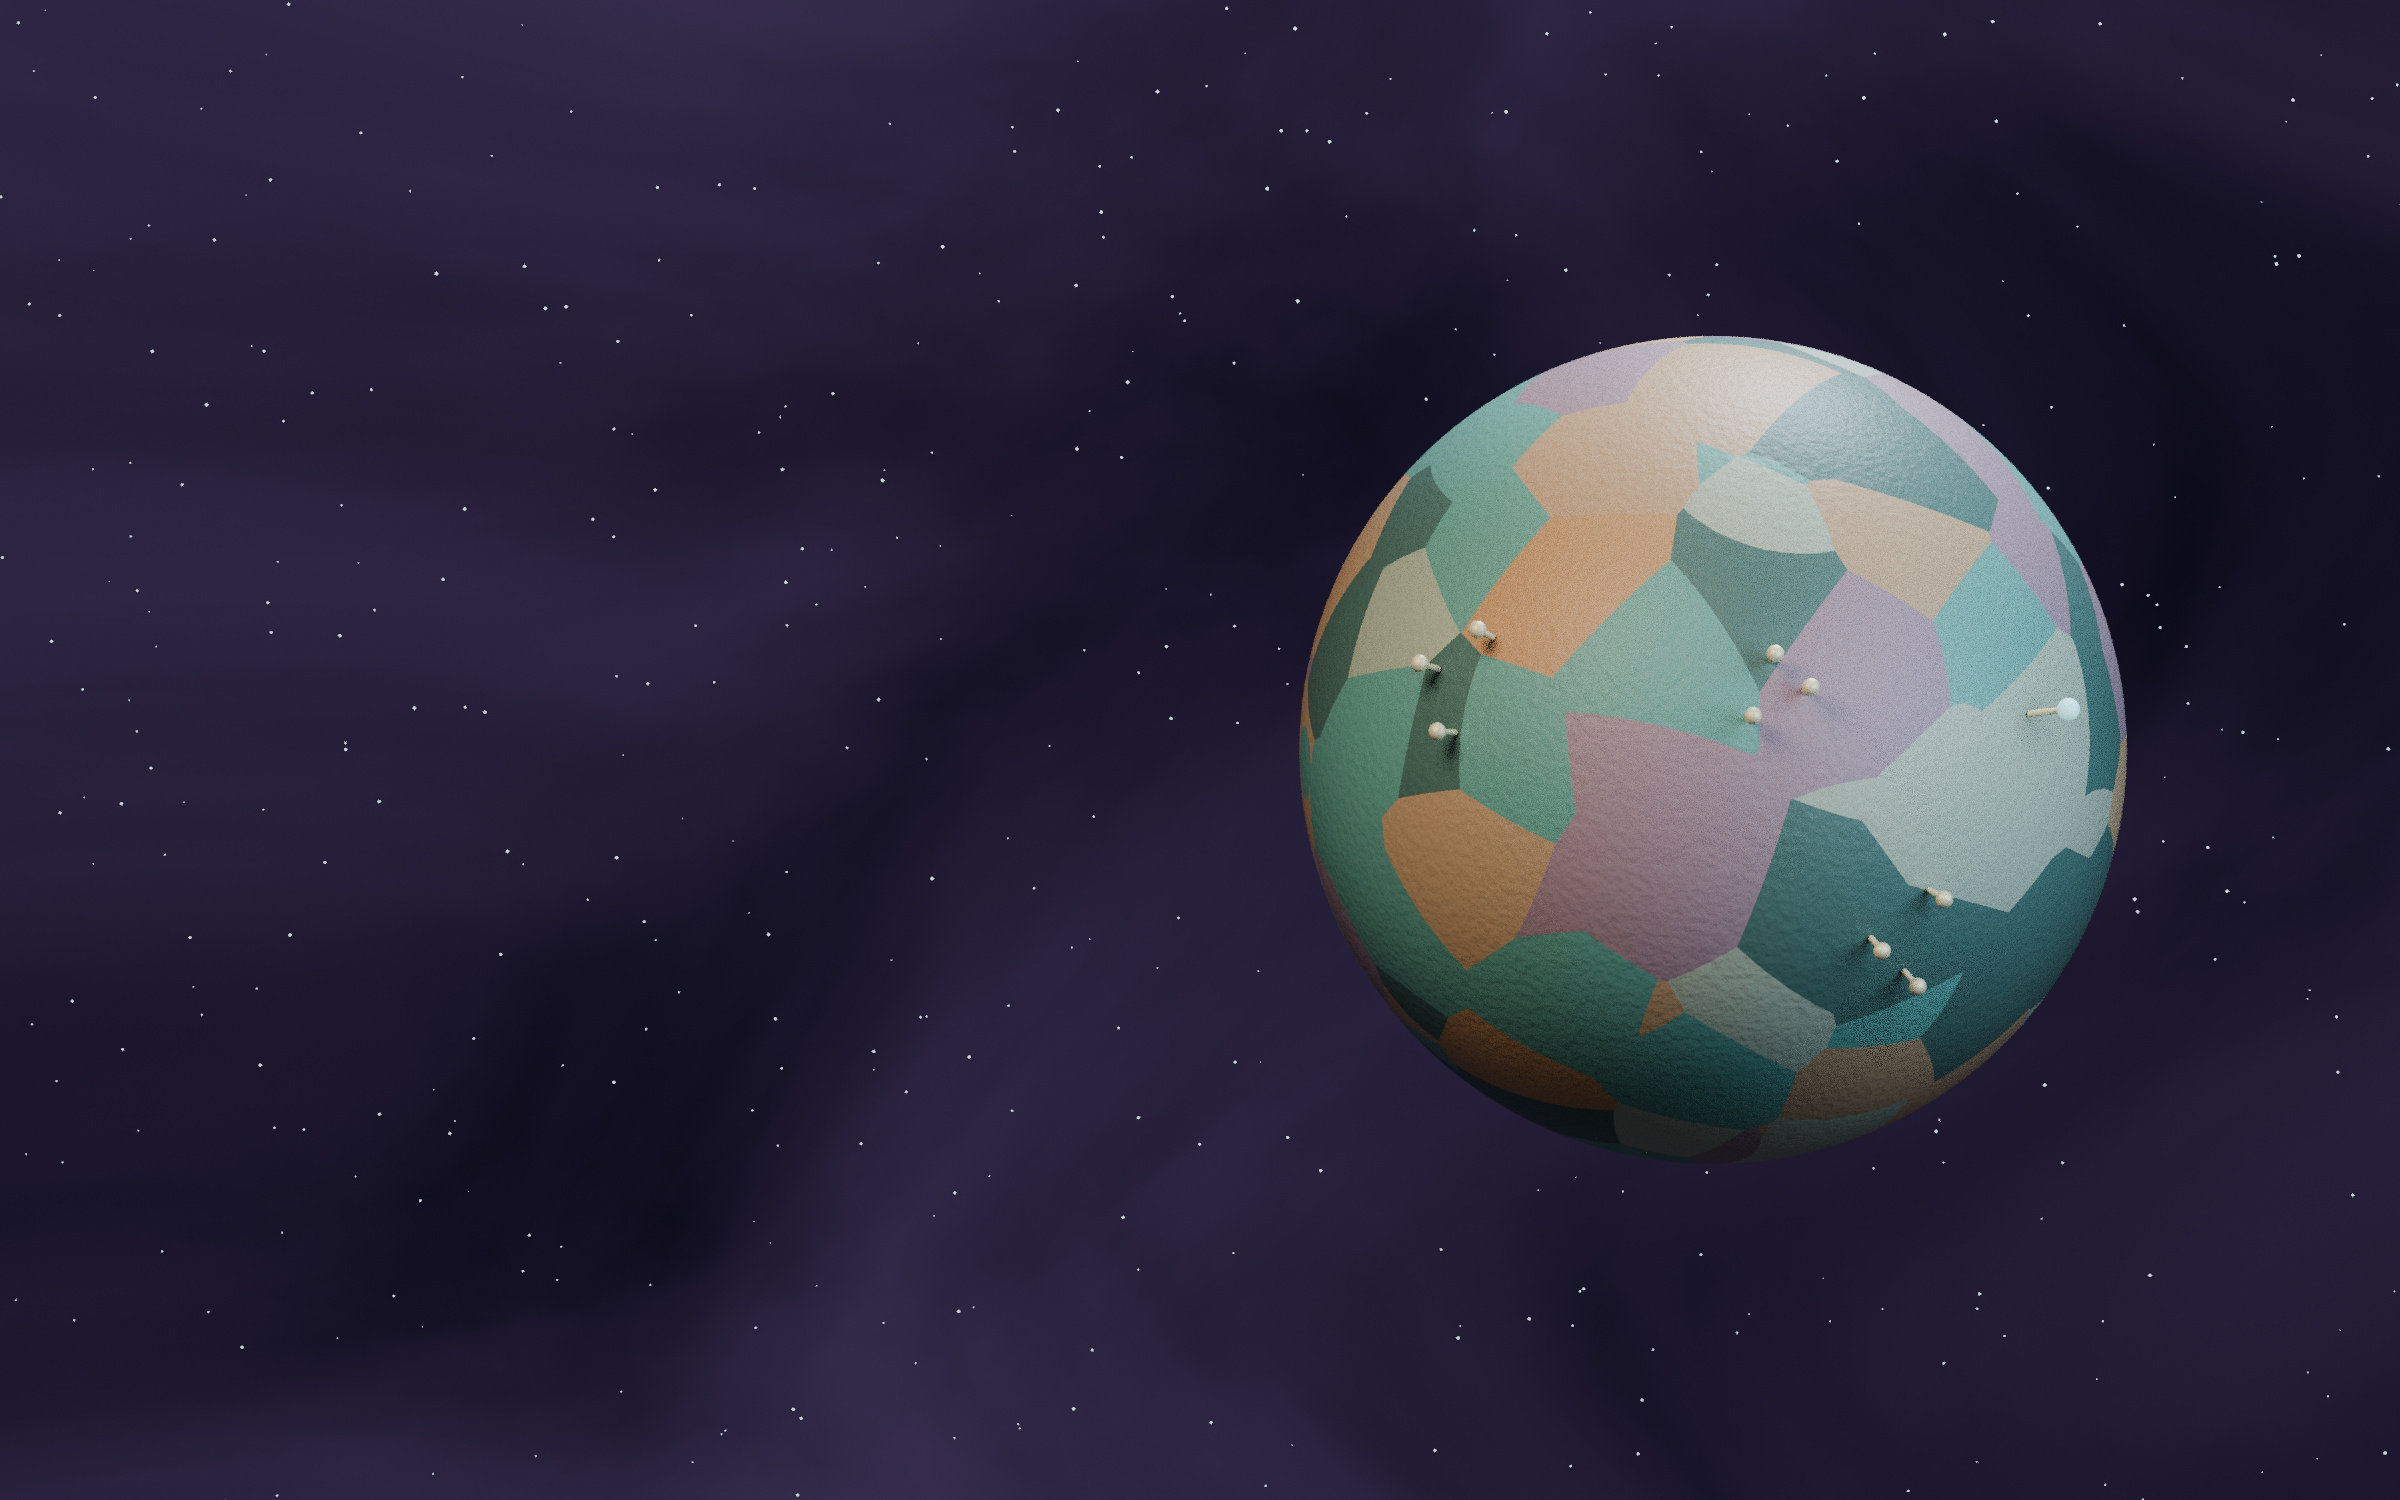
\includegraphics[width=20cm,height=12.5cm]{Scena/copertina.jpg}};}{}
\node[anchor=north west,inner sep=0] at([xshift=1.05cm,yshift=-1.10cm]current page.north west){\color{Mint}\bfseries\fontsize{23}{28}\selectfont PRISMA};
\node[anchor=north west,inner sep=0] at([xshift=1.07cm,yshift=-2.16cm]current page.north west){\color{white}\fontsize{9}{12}\selectfont MODULO M16 · SCIENZE DELLA TERRA};
\draw[Mint,line width=1.5pt]([xshift=1.07cm,yshift=-2.78cm]current page.north west)--([xshift=2.6cm,yshift=-2.78cm]current page.north west);
\node[anchor=north west,inner sep=0] at([xshift=1.05cm,yshift=-3.35cm]current page.north west){\begin{minipage}{9.2cm}\raggedright\color{white}\bfseries\fontsize{28.5}{34.5}\selectfont Classificazione\\e validazione\end{minipage}};
\node[anchor=north west,inner sep=0] at([xshift=1.07cm,yshift=-7.88cm]current page.north west){\begin{minipage}{8.9cm}\raggedright\color{Lilac}\fontsize{12.2}{17}\selectfont Riconoscere la litologia di una stazione nuova\end{minipage}};
\node[anchor=north west,inner sep=0] at([xshift=1.07cm,yshift=-8.70cm]current page.north west){\begin{minipage}{8.9cm}\raggedright\color{white!75}\fontsize{10.3}{14.5}\selectfont Confini decisionali, probabilità e trasferibilità\end{minipage}};
\node[anchor=north west,inner sep=0] at([xshift=1.07cm,yshift=-10.52cm]current page.north west){\color{white}\fontsize{10.5}{14}\selectfont GeoStat Lab · corso di Marzio De Corato};
\node[anchor=north west,inner sep=0] at([xshift=1.07cm,yshift=-11.17cm]current page.north west){\color{Mint}\fontsize{8.8}{11}\selectfont\href{https://creativecommons.org/licenses/by-nc-sa/4.0/}{Impaginazione da Tessera · CC BY-NC-SA 4.0}};
\end{tikzpicture}\end{frame}
\begin{frame}[plain]\hypertarget{slide2}{}
\bookmark[level=1,page=2]{Indice della presentazione}
\begin{tikzpicture}[remember picture,overlay]
\PilotChrome{Indice della presentazione}{PERCORSO}{2}{I titoli dell’indice aprono i capitoli. Il nome del capitolo in alto riporta a questa pagina.}
\node[anchor=north west,inner sep=0] at([xshift=.96cm,yshift=-2.12cm]current page.north west){\Colonna{9.40cm}{\PLabel{Capitoli}
{\fontsize{10.7}{13.5}\selectfont\hyperlink{slide4}{Campione e domanda predittiva\hfill 4}\par}\vspace{.16cm}
{\fontsize{10.7}{13.5}\selectfont\hyperlink{slide14}{Trasformazioni e geometria della decisione\hfill 14}\par}\vspace{.16cm}
{\fontsize{10.7}{13.5}\selectfont\hyperlink{slide25}{Selezione e validazione per gruppi\hfill 25}\par}\vspace{.16cm}
{\fontsize{10.7}{13.5}\selectfont\hyperlink{slide33}{Alberi e insiemi di classificatori\hfill 33}\par}\vspace{.16cm}
{\fontsize{10.7}{13.5}\selectfont\hyperlink{slide40}{Metriche e probabilità\hfill 40}\par}\vspace{.16cm}
{\fontsize{10.7}{13.5}\selectfont\hyperlink{slide54}{Diagnostica e trasferibilità\hfill 54}\par}\vspace{.16cm}
}};
\node[anchor=north west,inner sep=0] at([xshift=10.85cm,yshift=-2.12cm]current page.north west){\Colonna{8.16cm}{\PLabel{Percorso di lettura}
\PBody{Il dataset sintetico contiene tre litologie, cinque predittori e una gerarchia di provini e stazioni. Il test assegnato conserva tre stazioni complete, per trenta provini.}
\PInfo{Le pagine Scenario A e Confronto riprendono gli esperimenti nel browser. I valori di partenza del simulatore possono differire dal caso guida.}
\href{https://marzione00.github.io/Lab_Geo/\#modulo-M16}{\color{Classical}\bfseries Apri gli esperimenti di Prisma}}};
\end{tikzpicture}\end{frame}

\begin{frame}[plain]\hypertarget{slide3}{}
\bookmark[level=1,page=3]{Quanto informa una classificazione corretta se la stazione del provino era già nel training?}
\begin{tikzpicture}[remember picture,overlay]
\PilotChrome{{\fontsize{15.3}{19}\selectfont Quanto informa una classificazione corretta se la stazione del provino era già nel training?}}{IL CASO GUIDA}{3}{Un provino e una stazione rappresentano livelli diversi della verifica.}
\node[anchor=north west,inner sep=0] at([xshift=.96cm,yshift=-2.12cm]current page.north west){\Colonna{9.40cm}{{\centering\resizebox{.97\linewidth}{!}{\begin{tikzpicture}[x=1cm,y=1cm]

\node[pNote,anchor=west] at(.2,4.45){Campioni della stessa stazione};
\foreach \x/\id/\col in {1.4/S1/GeoA,4.1/S2/GeoA,6.8/S3/GeoB}{
 \draw[\col,fill=\col!8,rounded corners=4pt] (\x-1.05,1.3) rectangle(\x+1.05,3.95);
 \node[font=\bfseries,text=\col] at(\x,3.55){\id};
 \foreach \a/\b in {-.45/2.8,.37/2.85,-.25/2.15,.4/1.85}{\fill[\col] (\x+\a,\b) circle(3.5pt);}}
\draw[GeoA,line width=1pt] (.35,.98)--(5.15,.98);
\draw[GeoB,line width=1pt] (5.75,.98)--(7.85,.98);
\node[pNote] at(2.75,.62){training};\node[pNote] at (6.8,.62){test};
\node[pNote] at (4,-.05){Schema di una separazione per stazioni.};

\end{tikzpicture}
}\par}
}};
\node[anchor=north west,inner sep=0] at([xshift=10.85cm,yshift=-2.12cm]current page.north west){\Colonna{8.16cm}{\PLabel{Il caso}
\PBody{Il dataset sintetico contiene tre litologie, cinque predittori e una gerarchia di provini e stazioni. Il test assegnato conserva tre stazioni complete, per trenta provini.}
\PInfo{Imposteremo una regola di riferimento, sceglieremo i parametri nel training e leggeremo errori e probabilità sul territorio escluso.}
}};
\end{tikzpicture}\end{frame}

\begin{frame}[plain]\hypertarget{slide4}{}
\bookmark[level=0,page=4]{Campione e domanda predittiva}
\bookmark[level=1,page=4]{Una nuova misura o una nuova stazione?}
\begin{tikzpicture}[remember picture,overlay]
\PilotChrome{Una nuova misura o una nuova stazione?}{CAMPIONE E DOMANDA PREDITTIVA}{4}{Se la previsione riguarda nuove stazioni, separa e valuta per stazione.}
\node[anchor=north west,inner sep=0] at([xshift=.96cm,yshift=-2.12cm]current page.north west){\Colonna{9.40cm}{\PLabel{Domanda}
\PBody{Se due provini della stazione S1 finiscono uno nel training e uno nel test, il modello è valutato su una stazione che ha già visto. Qual è l’unità di trasferimento?}
\vspace{.35cm}\PLabel{Interpretazione}
\PBody{Il confronto fra gli insiemi di stazioni segnala ogni sovrapposizione. Lo stesso controllo sugli identificativi dei singoli provini perderebbe la dipendenza.}
}};
\node[anchor=north west,inner sep=0] at([xshift=10.85cm,yshift=-2.12cm]current page.north west){\Colonna{8.16cm}{\begin{tcolorbox}[enhanced,arc=1.7mm,boxrule=.6pt,colback=white,colframe=Classical!60!Navy,colbacktitle=Navy,coltitle=white,fonttitle=\bfseries\small,title={R · calcolo riproducibile},left=1.7mm,right=1.3mm,top=1.1mm,bottom=1.1mm,before skip=1mm,after skip=1.0mm]\lstinputlisting[style=GeoR,language=R]{Codice/capitolo-01.R}\end{tcolorbox}
\PLabel{Risultato in R}
\begin{tcolorbox}[colback=GeoTint,colframe=Rule,boxrule=.5pt,arc=1.4mm,left=2mm,right=1mm,top=1mm,bottom=1mm]{\fontsize{9}{12}\selectfont\ttfamily \mbox{[1]\ "S2"}}\end{tcolorbox}}};
\end{tikzpicture}\end{frame}

\begin{frame}[plain]\hypertarget{slide5}{}
\bookmark[level=1,page=5]{Classificare campioni entro un dominio definito}
\begin{tikzpicture}[remember picture,overlay]
\PilotChrome{Classificare campioni entro un dominio definito}{CAMPIONE E DOMANDA PREDITTIVA}{5}{La domanda predittiva comprende le classi, le misure disponibili e la popolazione di applicazione.}
\node[anchor=north west,inner sep=0] at([xshift=.96cm,yshift=-2.12cm]current page.north west){\Colonna{9.40cm}{{\centering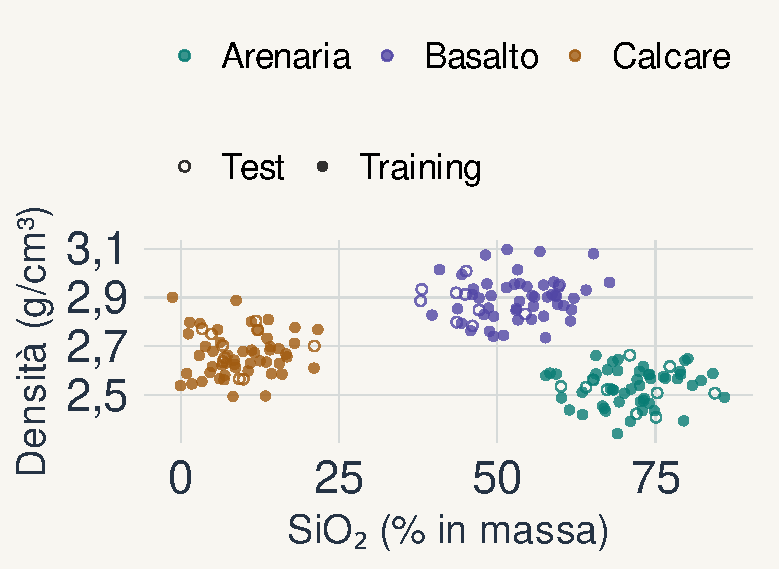
\includegraphics[width=\linewidth,height=6.15cm,keepaspectratio]{Figure/F01.pdf}\par}
\PSmall{Vista di due predittori fra i cinque disponibili. I simboli distinguono campioni di addestramento e di test.}
}};
\node[anchor=north west,inner sep=0] at([xshift=10.85cm,yshift=-2.12cm]current page.north west){\Colonna{8.16cm}{\PBody{La classificazione associa un insieme di misure a una classe, utilizzando esempi nei quali la risposta è già disponibile. Il dataset didattico contiene centottanta campioni sintetici, raccolti idealmente in diciotto stazioni e suddivisi fra Arenaria, Basalto e Calcare. Quattro variabili composizionali e la densità costituiscono i predittori. Le etichette e la separazione fra gruppi derivano dal generatore della simulazione, per cui le prestazioni misurano il comportamento entro questo esercizio e richiedono nuove evidenze prima di un impiego su campioni reali.}
}};
\end{tikzpicture}\end{frame}

\begin{frame}[plain]\hypertarget{slide6}{}
\bookmark[level=1,page=6]{Rischio predittivo e distribuzione di applicazione}
\begin{tikzpicture}[remember picture,overlay]
\PilotChrome{Rischio predittivo e distribuzione di applicazione}{CAMPIONE E DOMANDA PREDITTIVA}{6}{La validità della valutazione dipende dalla corrispondenza fra test e contesto di applicazione.}
\node[anchor=north west,inner sep=0] at([xshift=.96cm,yshift=-2.12cm]current page.north west){\Colonna{9.40cm}{\PLabel{Metodo}
\PBody{Una regola appresa viene valutata mediante la perdita su nuovi casi della popolazione di interesse. Con perdita zero–uno, il rischio corrisponde alla probabilità di classificazione errata. La media degli errori sul test è una stima riferita alla distribuzione rappresentata da quei dati, la cui pertinenza dipende dal modo in cui sono stati raccolti e separati. Cambiamenti di strumento, ambiente o classi possono richiedere una nuova valutazione.}
}};
\node[anchor=north west,inner sep=0] at([xshift=10.85cm,yshift=-2.12cm]current page.north west){\Colonna{8.16cm}{\PLabel{Formalismo}
\par\smallskip{\centering\adjustbox{max width=.98\linewidth}{$\displaystyle R(f)=E\!\left[\mathbf1\{f(X)\ne Y\}\right]$}\par\smallskip}

\par\smallskip{\centering\adjustbox{max width=.98\linewidth}{$\displaystyle \widehat R_{test}=\frac1{n_{test}}\sum_i\mathbf1\{f(x_i)\ne y_i\}$}\par\smallskip}
\PLabel{Interpretazione}
\PBody{X è il vettore dei predittori; Y la classe; f la regola già appresa. L’attesa riguarda nuovi casi della popolazione di applicazione. Nel test, $(x_i,y_i)$ sono i casi osservati e $n_{\rm test}$ la loro numerosità. Se più provini appartengono alla stessa stazione, la dipendenza entra nel disegno di validazione e nella quantificazione dell’incertezza.}
}};
\end{tikzpicture}\end{frame}

\begin{frame}[plain]\hypertarget{slide7}{}
\bookmark[level=1,page=7]{Provini e stazioni come livelli del campionamento}
\begin{tikzpicture}[remember picture,overlay]
\PilotChrome{Provini e stazioni come livelli del campionamento}{CAMPIONE E DOMANDA PREDITTIVA}{7}{L’unità di separazione deve riflettere l’unità sulla quale si vuole valutare la generalizzazione.}
\node[anchor=north west,inner sep=0] at([xshift=.96cm,yshift=-2.12cm]current page.north west){\Colonna{9.40cm}{{\centering\resizebox{.97\linewidth}{!}{\begin{tikzpicture}[x=1cm,y=-.87cm,every node/.style={font=\fontsize{12.2}{15}\selectfont,text=Ink},arr/.style={-{Stealth[length=2mm]},line width=.8pt,draw=Classical}]\path[use as bounding box] (0,0) rectangle (7.45,6.2);
\draw[draw=Classical,fill=Classical!8,rounded corners=2pt,line width=.7pt] (0.5,0.6) rectangle (6.9,1.7);
\node[anchor=center,text=Ink,font=\fontsize{12.2}{15}\selectfont,text width=6cm,align=center] at (3.7,1.15) {Una stazione: condizioni condivise};
\draw[arr,draw=Classical] (1.7,1.9)--(1.7,3);
\draw[arr,draw=Classical] (3.7,1.9)--(3.7,3);
\draw[arr,draw=Classical] (5.7,1.9)--(5.7,3);
\draw[draw=Classical,fill=Classical!8,rounded corners=2pt,line width=.7pt] (0.9,3.2) rectangle (2.5,4.5);
\node[anchor=center,text=Ink,font=\fontsize{11}{15}\selectfont,text width=1.4cm,align=center] at (1.7000000000000002,3.85) {Provino A};
\draw[draw=Classical,fill=Classical!8,rounded corners=2pt,line width=.7pt] (2.9,3.2) rectangle (4.5,4.5);
\node[anchor=center,text=Ink,font=\fontsize{11}{15}\selectfont,text width=1.4cm,align=center] at (3.7,3.85) {Provino B};
\draw[draw=Classical,fill=Classical!8,rounded corners=2pt,line width=.7pt] (4.9,3.2) rectangle (6.5,4.5);
\node[anchor=center,text=Ink,font=\fontsize{11}{15}\selectfont,text width=1.4cm,align=center] at (5.7,3.85) {Provino C};
\node[anchor=center,text=Ink,font=\fontsize{12.2}{15}\selectfont,text width=6.7cm,align=center] at (3.7,5.5) {Il gruppo resta unito nella validazione.};

\end{tikzpicture}}\par}
}};
\node[anchor=north west,inner sep=0] at([xshift=10.85cm,yshift=-2.12cm]current page.north west){\Colonna{8.16cm}{\PBody{L’identificativo è unico per ogni provino, mentre il codice di stazione compare dieci volte perché descrive il raggruppamento delle misure. Questa ripetizione conserva informazione sul disegno di raccolta. Una separazione casuale delle righe potrebbe distribuire provini della stessa stazione fra addestramento e test, favorendo una valutazione legata a condizioni locali già osservate. Per esaminare il trasferimento a stazioni ulteriori, tutti i provini di una stazione vengono assegnati allo stesso insieme.}
}};
\end{tikzpicture}\end{frame}

\begin{frame}[plain]\hypertarget{slide8}{}
\bookmark[level=1,page=8]{La separazione prestabilita per stazioni}
\begin{tikzpicture}[remember picture,overlay]
\PilotChrome{La separazione prestabilita per stazioni}{CAMPIONE E DOMANDA PREDITTIVA}{8}{I trenta provini di test appartengono a tre stazioni e conservano questa struttura nella lettura delle prestazioni.}
\node[anchor=north west,inner sep=0] at([xshift=.96cm,yshift=-2.12cm]current page.north west){\Colonna{9.40cm}{\begin{tcolorbox}[enhanced,arc=1.7mm,boxrule=.6pt,colback=white,colframe=Classical!60!Navy,colbacktitle=Navy,coltitle=white,fonttitle=\bfseries\small,title={R · procedura},left=1.7mm,right=1.3mm,top=1.1mm,bottom=1.1mm,before skip=1mm,after skip=1.0mm]\lstinputlisting[style=GeoR,language=R]{Codice/lettura-06.R}\end{tcolorbox}
}};
\node[anchor=north west,inner sep=0] at([xshift=10.85cm,yshift=-2.12cm]current page.north west){\Colonna{8.16cm}{\PBody{Le stazioni con suffisso sei costituiscono il test, mentre le altre cinque stazioni di ciascuna classe alimentano l’addestramento. Si ottengono centocinquanta campioni in quindici stazioni e trenta campioni in tre stazioni, con dieci osservazioni per classe nel test. Il controllo verifica disgiunzione e conteggi senza estrarre una nuova divisione a ogni esecuzione. La presenza di una sola stazione di test per classe limita l’informazione sulla variabilità fra stazioni, anche quando tutti i provini vengono classificati correttamente.}
}};
\end{tikzpicture}\end{frame}

\begin{frame}[plain]\hypertarget{slide9}{}
\bookmark[level=1,page=9]{Le righe del CSV rappresentano provini raggruppati}
\begin{tikzpicture}[remember picture,overlay]
\PilotChrome{Le righe del CSV rappresentano provini raggruppati}{CAMPIONE E DOMANDA PREDITTIVA}{9}{Il conteggio descrive l’equilibrio delle etichette.}
\node[anchor=north west,inner sep=0] at([xshift=.96cm,yshift=-2.12cm]current page.north west){\Colonna{9.40cm}{\PLabel{Risultati del calcolo in R}
{\fontsize{10.2}{12.8}\selectfont\begin{tabular}{@{}>{\raggedright\arraybackslash}p{0.31\linewidth}@{\hspace{.13cm}}>{\raggedright\arraybackslash}p{0.29\linewidth}@{\hspace{.13cm}}>{\raggedright\arraybackslash}p{0.32\linewidth}@{}}\toprule litologia & split & Numero\\[2.3pt]
\midrule 
Arenaria & test & 10\\[2.3pt]
Basalto & test & 10\\[2.3pt]
Arenaria & train & 50\\[2.3pt]
Basalto & train & 50\\[2.3pt]
Calcare & train & 50\\[2.3pt]
\bottomrule\end{tabular}\par}
\PSmall{Selezione di cinque righe dal file completo.}
}};
\node[anchor=north west,inner sep=0] at([xshift=10.85cm,yshift=-2.12cm]current page.north west){\Colonna{8.16cm}{\PBody{Quanti provini di ciascuna litologia entrano negli insiemi di sviluppo e verifica?}
\vspace{.4cm}\PInfo{Il conteggio descrive l’equilibrio delle etichette. Per comprendere l’indipendenza della prova bisogna contare anche le stazioni.}
}};
\node[anchor=north east,inner sep=0] at([xshift=17.1cm,yshift=-12.04cm]current page.north west){\fontsize{7.7}{9}\selectfont \href{https://github.com/marzione00/Lab_Geo/blob/649f7cc577b96bd1044d81e78a2f530813e4f96b/materiali/laboratori/M16/M16_N01.R}{\color{Classical}\bfseries Script R · M16\_N01}};
\end{tikzpicture}\end{frame}

\begin{frame}[plain]\hypertarget{slide10}{}
\bookmark[level=1,page=10]{Il numero di stazioni descrive il test esterno}
\begin{tikzpicture}[remember picture,overlay]
\PilotChrome{Il numero di stazioni descrive il test esterno}{CAMPIONE E DOMANDA PREDITTIVA}{10}{Il training contiene 150 provini distribuiti su 15 stazioni.}
\node[anchor=north west,inner sep=0] at([xshift=.96cm,yshift=-2.12cm]current page.north west){\Colonna{9.40cm}{\PLabel{Risultati del calcolo in R}
{\fontsize{10.2}{12.8}\selectfont\begin{tabular}{@{}>{\raggedright\arraybackslash}p{0.31\linewidth}@{\hspace{.13cm}}>{\raggedright\arraybackslash}p{0.29\linewidth}@{\hspace{.13cm}}>{\raggedright\arraybackslash}p{0.32\linewidth}@{}}\toprule set & campioni & stazioni\\[2.3pt]
\midrule 
train & 150 & 15\\[2.3pt]
test & 30 & 3\\[2.3pt]
\bottomrule\end{tabular}\par}
}};
\node[anchor=north west,inner sep=0] at([xshift=10.85cm,yshift=-2.12cm]current page.north west){\Colonna{8.16cm}{\PBody{Quante unità geologiche indipendenti sostengono il risultato finale?}
\vspace{.4cm}\PInfo{Il training contiene 150 provini distribuiti su 15 stazioni. Il test comprende 30 provini di sole tre stazioni. I due conteggi raccontano livelli di replica diversi.}
}};
\node[anchor=north east,inner sep=0] at([xshift=17.1cm,yshift=-12.04cm]current page.north west){\fontsize{7.7}{9}\selectfont \href{https://github.com/marzione00/Lab_Geo/blob/649f7cc577b96bd1044d81e78a2f530813e4f96b/materiali/laboratori/M16/M16_N02.R}{\color{Classical}\bfseries Script R · M16\_N02}};
\end{tikzpicture}\end{frame}

\begin{frame}[plain]\hypertarget{slide11}{}
\bookmark[level=1,page=11]{Una regola costante dà il riferimento di partenza}
\begin{tikzpicture}[remember picture,overlay]
\PilotChrome{Una regola costante dà il riferimento di partenza}{CAMPIONE E DOMANDA PREDITTIVA}{11}{Nel test bilanciato la regola raggiunge un terzo di accuratezza.}
\node[anchor=north west,inner sep=0] at([xshift=.96cm,yshift=-2.12cm]current page.north west){\Colonna{9.40cm}{\PLabel{Risultati del calcolo in R}
{\fontsize{10.2}{12.8}\selectfont\begin{tabular}{@{}>{\raggedright\arraybackslash}p{0.52\linewidth}@{\hspace{.13cm}}>{\raggedright\arraybackslash}p{0.39\linewidth}@{}}\toprule Grandezza & Valore\\[2.3pt]
\midrule 
regola & maggioranza training\\[2.3pt]
classe & Arenaria\\[2.3pt]
Accuratezza & 0,33333\\[2.3pt]
\bottomrule\end{tabular}\par}
}};
\node[anchor=north west,inner sep=0] at([xshift=10.85cm,yshift=-2.12cm]current page.north west){\Colonna{8.16cm}{\PBody{Quanto ottiene il classificatore che assegna la classe più frequente del training?}
\vspace{.4cm}\PInfo{Nel test bilanciato la regola raggiunge un terzo di accuratezza. Un modello più elaborato va giudicato rispetto a un riferimento esplicito.}
}};
\node[anchor=north east,inner sep=0] at([xshift=17.1cm,yshift=-12.04cm]current page.north west){\fontsize{7.7}{9}\selectfont \href{https://github.com/marzione00/Lab_Geo/blob/649f7cc577b96bd1044d81e78a2f530813e4f96b/materiali/laboratori/M16/M16_N03.R}{\color{Classical}\bfseries Script R · M16\_N03}};
\end{tikzpicture}\end{frame}

\begin{frame}[plain]\hypertarget{slide12}{}
\bookmark[level=1,page=12]{Bersaglio predittivo e nuove stazioni}
\begin{tikzpicture}[remember picture,overlay]
\PilotChrome{Bersaglio predittivo e nuove stazioni}{CAMPIONE E DOMANDA PREDITTIVA}{12}{Confrontare predizione di misure e trasferimento a nuove unità.}
\node[anchor=north west,inner sep=0] at([xshift=.96cm,yshift=-2.12cm]current page.north west){\Colonna{9.40cm}{{\centering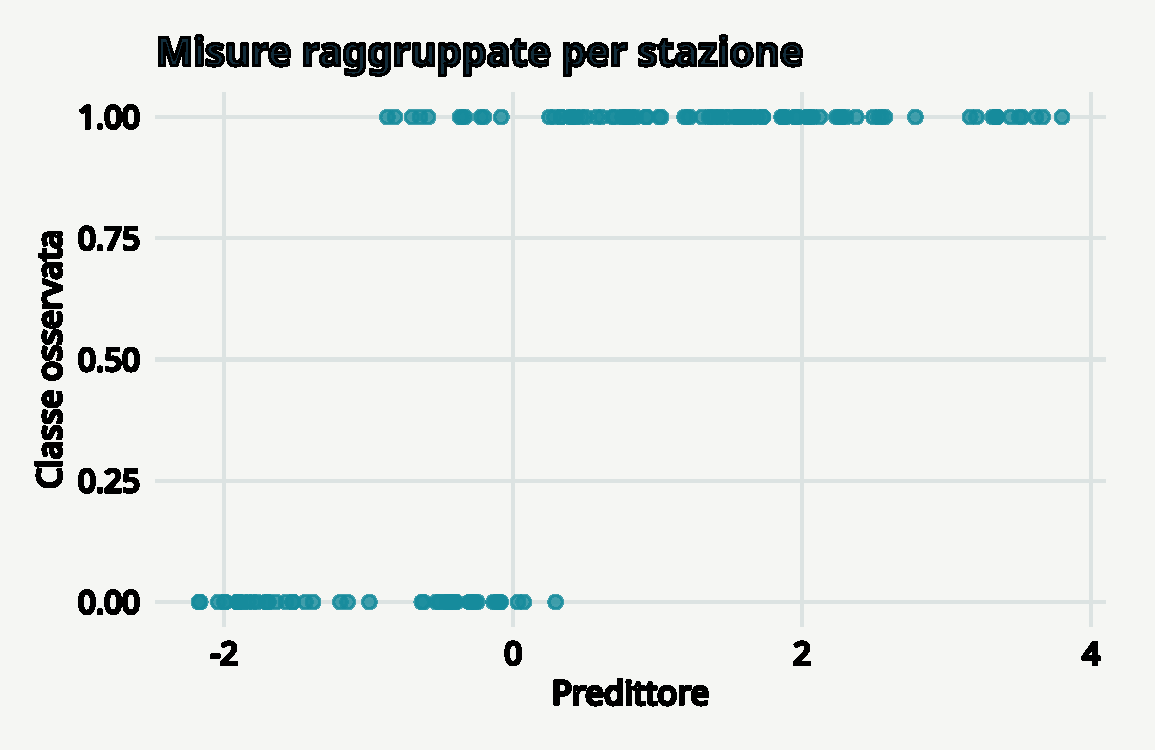
\includegraphics[width=\linewidth,height=6.0cm,keepaspectratio]{Esperimenti/m16-bersaglio-A.pdf}\par}
\PSmall{Ampiezza dell’effetto di stazione: 2. Seme: 17.}
}};
\node[anchor=north west,inner sep=0] at([xshift=10.85cm,yshift=-2.12cm]current page.north west){\Colonna{8.16cm}{\PLabel{Scenario A · simulazione}
\PBody{La validazione di un classificatore deve rappresentare il tipo di osservazione che incontrerà nell’uso futuro. L’esperimento genera misure raggruppate per stazione, con un effetto condiviso che contribuisce sia al predittore sia alla probabilità della classe. Un classificatore a un vicino viene valutato mediante una separazione casuale delle misure e mediante stazioni interamente escluse dall’addestramento.}
\par\smallskip{\centering\adjustbox{max width=.98\linewidth}{$\displaystyle \widehat R=\frac1{n_{test}}\sum_i\mathbf1(\widehat y_i\ne y_i)$}\par\smallskip}
\PSmall{$\hat y_i$ è la classe prevista, $y_i$ quella osservata e $n_{\mathrm{test}}$ il numero di misure escluse dall’addestramento. $\hat R$ è la frequenza degli errori; le metriche dell’interfaccia riportano l’accuratezza, pari a $1-\hat R$.}
}};
\node[anchor=north east,inner sep=0] at([xshift=17.1cm,yshift=-12.04cm]current page.north west){\fontsize{7.7}{9}\selectfont \href{https://marzione00.github.io/Lab_Geo/\#laboratorio/m16-bersaglio}{\color{Classical}\bfseries Apri il laboratorio · m16-bersaglio}};
\end{tikzpicture}\end{frame}

\begin{frame}[plain]\hypertarget{slide13}{}
\bookmark[level=1,page=13]{Confronto | Bersaglio predittivo e nuove stazioni}
\begin{tikzpicture}[remember picture,overlay]
\PilotChrome{Confronto | Bersaglio predittivo e nuove stazioni}{CAMPIONE E DOMANDA PREDITTIVA}{13}{Il protocollo di verifica deve corrispondere all’unità che sarà incontrata nell’uso futuro.}
\node[anchor=north west,inner sep=0] at([xshift=.96cm,yshift=-2.12cm]current page.north west){\Colonna{9.40cm}{{\centering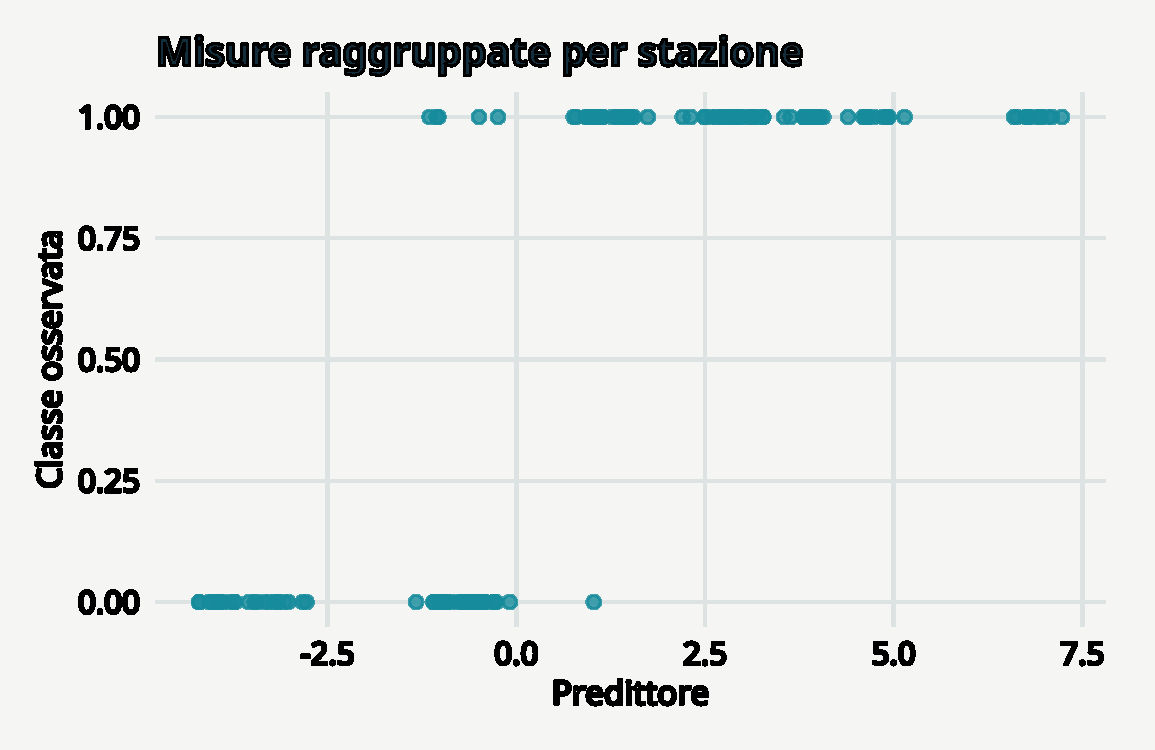
\includegraphics[width=\linewidth,height=5.6cm,keepaspectratio]{Esperimenti/m16-bersaglio-B.pdf}\par}
\PSmall{Ampiezza dell’effetto di stazione: 2 $\to$ 4. Tutti gli altri parametri e il seme sono fissi.}
}};
\node[anchor=north west,inner sep=0] at([xshift=10.85cm,yshift=-2.12cm]current page.north west){\Colonna{8.16cm}{\PLabel{Confronto fra gli scenari}
{\fontsize{10.2}{12.8}\selectfont\begin{tabular}{@{}>{\raggedright\arraybackslash}p{0.48\linewidth}@{\hspace{.13cm}}>{\raggedright\arraybackslash}p{0.224\linewidth}@{\hspace{.13cm}}>{\raggedright\arraybackslash}p{0.224\linewidth}@{}}\toprule Grandezza & A & B\\[2.3pt]
\midrule 
Accuratezza separazione casuale & 0,958 & 0,896\\[2.3pt]
Accuratezza nuove stazioni & 0,75 & 0,729\\[2.3pt]
Stazioni complessive & 12 & 12\\[2.3pt]
\bottomrule\end{tabular}\par}
\vspace{.25cm}\PBody{In entrambi gli scenari l’accuratezza scende quando si escludono stazioni intere. Le prestazioni dipendono dall’unità con cui si costruisce il test.}
}};
\node[anchor=north east,inner sep=0] at([xshift=17.1cm,yshift=-12.04cm]current page.north west){\fontsize{7.7}{9}\selectfont \href{https://marzione00.github.io/Lab_Geo/\#laboratorio/m16-bersaglio}{\color{Classical}\bfseries Apri il laboratorio · m16-bersaglio}};
\end{tikzpicture}\end{frame}

\begin{frame}[plain]\hypertarget{slide14}{}
\bookmark[level=0,page=14]{Trasformazioni e geometria della decisione}
\bookmark[level=1,page=14]{La scala del nuovo campione viene dal training}
\begin{tikzpicture}[remember picture,overlay]
\PilotChrome{La scala del nuovo campione viene dal training}{TRASFORMAZIONI E GEOMETRIA DELLA DECISIONE}{14}{Stima ogni trasformazione sui dati disponibili prima della previsione.}
\node[anchor=north west,inner sep=0] at([xshift=.96cm,yshift=-2.12cm]current page.north west){\Colonna{9.40cm}{\PLabel{Domanda}
\PBody{Una variabile del training ha valori 10, 12 e 14. Una nuova stazione dà 16. Usiamo media e deviazione standard campionaria del training.}
\vspace{.35cm}\PLabel{Interpretazione}
\PBody{La media è 12 e la deviazione standard è 2. Il nuovo campione si trova due deviazioni standard sopra il centro del training.}
}};
\node[anchor=north west,inner sep=0] at([xshift=10.85cm,yshift=-2.12cm]current page.north west){\Colonna{8.16cm}{\begin{tcolorbox}[enhanced,arc=1.7mm,boxrule=.6pt,colback=white,colframe=Classical!60!Navy,colbacktitle=Navy,coltitle=white,fonttitle=\bfseries\small,title={R · calcolo riproducibile},left=1.7mm,right=1.3mm,top=1.1mm,bottom=1.1mm,before skip=1mm,after skip=1.0mm]\lstinputlisting[style=GeoR,language=R]{Codice/capitolo-02.R}\end{tcolorbox}
\PLabel{Risultato in R}
\begin{tcolorbox}[colback=GeoTint,colframe=Rule,boxrule=.5pt,arc=1.4mm,left=2mm,right=1mm,top=1mm,bottom=1mm]{\fontsize{9}{12}\selectfont\ttfamily \mbox{centro\ \ \ scala\ z\_nuovo\ }\\\mbox{\ \ \ \ \ 12\ \ \ \ \ \ \ 2\ \ \ \ \ \ \ 2}}\end{tcolorbox}}};
\end{tikzpicture}\end{frame}

\begin{frame}[plain]\hypertarget{slide15}{}
\bookmark[level=1,page=15]{Una regola di riferimento prima dei modelli}
\begin{tikzpicture}[remember picture,overlay]
\PilotChrome{Una regola di riferimento prima dei modelli}{TRASFORMAZIONI E GEOMETRIA DELLA DECISIONE}{15}{Il riferimento rende interpretabile il miglioramento ottenuto mediante le variabili predittive.}
\node[anchor=north west,inner sep=0] at([xshift=.96cm,yshift=-2.12cm]current page.north west){\Colonna{9.40cm}{{\centering\resizebox{.97\linewidth}{!}{\begin{tikzpicture}[x=1cm,y=-.87cm,every node/.style={font=\fontsize{12.2}{15}\selectfont,text=Ink},arr/.style={-{Stealth[length=2mm]},line width=.8pt,draw=Classical}]\path[use as bounding box] (0,0) rectangle (7.45,6.2);
\draw[draw=Classical,fill=Classical!8,rounded corners=2pt,line width=.7pt] (0.5,0.4) rectangle (6.9,1.5499999999999998);
\node[anchor=center,text=Ink,font=\fontsize{11.5}{15}\selectfont,text width=6cm,align=center] at (3.7,0.975) {Frequenze nel solo addestramento};
\draw[arr,draw=Classical] (3.7,1.7000000000000002)--(3.7,2.08);
\draw[draw=Quantum,fill=Quantum!8,rounded corners=2pt,line width=.7pt] (0.5,2.25) rectangle (6.9,3.4);
\node[anchor=center,text=Ink,font=\fontsize{11.5}{15}\selectfont,text width=6cm,align=center] at (3.7,2.825) {Regola dichiarata per il pareggio};
\draw[arr,draw=Classical] (3.7,3.55)--(3.7,3.9299999999999997);
\draw[draw=Classical,fill=Classical!8,rounded corners=2pt,line width=.7pt] (0.5,4.1000000000000005) rectangle (6.9,5.25);
\node[anchor=center,text=Ink,font=\fontsize{11.5}{15}\selectfont,text width=6cm,align=center] at (3.7,4.675000000000001) {Predizione costante: Arenaria};

\end{tikzpicture}}\par}
\PSmall{$n_{c,train}$: casi della classe c nell’addestramento; $\widehat y$: classe assegnata. Acc è la frazione di classificazioni corrette.}
}};
\node[anchor=north west,inner sep=0] at([xshift=10.85cm,yshift=-2.12cm]current page.north west){\Colonna{8.16cm}{\PBody{La classe più frequente nell’addestramento fornisce una regola elementare con cui confrontare il valore aggiunto dei predittori. Poiché le tre classi hanno cinquanta campioni ciascuna, il laboratorio risolve il pareggio mediante l’ordine alfabetico e assegna Arenaria a tutti i casi. Nel test bilanciato la regola ottiene dieci classificazioni corrette su trenta, pari a un terzo. Anche questo riferimento viene definito utilizzando soltanto l’addestramento, affinché il confronto rispetti il medesimo protocollo dei modelli più articolati.}
\par\smallskip{\centering\adjustbox{max width=.98\linewidth}{$\displaystyle \widehat y=\arg\max_c n_{c,train},\qquad Acc_{test}=\frac{10}{30}$}\par\smallskip}
}};
\end{tikzpicture}\end{frame}

\begin{frame}[plain]\hypertarget{slide16}{}
\bookmark[level=1,page=16]{Una scala comune stimata sull’addestramento}
\begin{tikzpicture}[remember picture,overlay]
\PilotChrome{Una scala comune stimata sull’addestramento}{TRASFORMAZIONI E GEOMETRIA DELLA DECISIONE}{16}{I parametri di ogni trasformazione appresa seguono il medesimo confine dei dati usati per adattare il modello.}
\node[anchor=north west,inner sep=0] at([xshift=.96cm,yshift=-2.12cm]current page.north west){\Colonna{9.40cm}{{\centering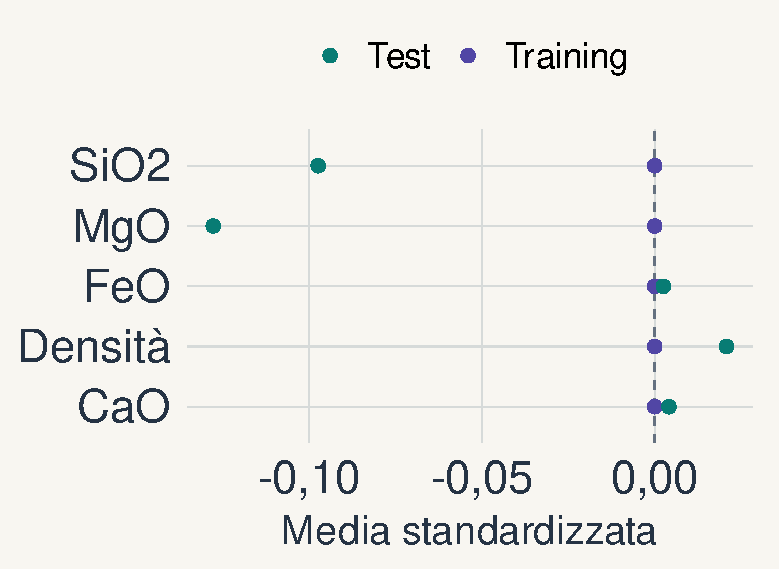
\includegraphics[width=\linewidth,height=6.15cm,keepaspectratio]{Figure/F02.pdf}\par}
\PSmall{$x_{ij}$: predittore j del caso i; $\bar x_{j,train}$ e $s_{j,train}$: media e deviazione nell’addestramento. z è adimensionale.}
}};
\node[anchor=north west,inner sep=0] at([xshift=10.85cm,yshift=-2.12cm]current page.north west){\Colonna{8.16cm}{\PBody{La standardizzazione sottrae la media e divide per la deviazione standard di ciascun predittore, entrambe stimate sull’addestramento. Gli stessi parametri vengono applicati ai campioni di test, che mantengono così il sistema di riferimento nel quale è stato adattato il modello. Le medie standardizzate del test possono essere diverse da zero, poiché descrivono osservazioni ulteriori. Una trasformazione calcolata separatamente sul test cambierebbe le coordinate ricevute dal classificatore e utilizzerebbe informazioni esterne al procedimento definito.}
\par\smallskip{\centering\adjustbox{max width=.98\linewidth}{$\displaystyle z_{ij}=\frac{x_{ij}-\overline x_{j,train}}{s_{j,train}},\qquad s_{j,train}>0$}\par\smallskip}
}};
\end{tikzpicture}\end{frame}

\begin{frame}[plain]\hypertarget{slide17}{}
\bookmark[level=1,page=17]{La trasformazione come oggetto da conservare}
\begin{tikzpicture}[remember picture,overlay]
\PilotChrome{La trasformazione come oggetto da conservare}{TRASFORMAZIONI E GEOMETRIA DELLA DECISIONE}{17}{Il modello distribuito comprende anche le trasformazioni necessarie a interpretarne gli input.}
\node[anchor=north west,inner sep=0] at([xshift=.96cm,yshift=-2.12cm]current page.north west){\Colonna{9.40cm}{\begin{tcolorbox}[enhanced,arc=1.7mm,boxrule=.6pt,colback=white,colframe=Classical!60!Navy,colbacktitle=Navy,coltitle=white,fonttitle=\bfseries\small,title={R · procedura},left=1.7mm,right=1.3mm,top=1.1mm,bottom=1.1mm,before skip=1mm,after skip=1.0mm]\lstinputlisting[style=GeoR,language=R]{Codice/lettura-09.R}\end{tcolorbox}
}};
\node[anchor=north west,inner sep=0] at([xshift=10.85cm,yshift=-2.12cm]current page.north west){\Colonna{8.16cm}{\PBody{Il codice separa la stima dei parametri dalla loro applicazione, rendendo ispezionabili media e deviazione standard. Questi oggetti devono essere conservati insieme al classificatore per trasformare ogni nuovo campione nello stesso modo. Il controllo della deviazione standard intercetta predittori costanti, per i quali la divisione sarebbe indefinita. L’esecuzione su una sessione pulita verifica inoltre che la trasformazione utilizzi i dati dichiarati e non valori rimasti nell’ambiente da un’analisi precedente.}
}};
\end{tikzpicture}\end{frame}

\begin{frame}[plain]\hypertarget{slide18}{}
\bookmark[level=1,page=18]{Il classificatore del centroide più vicino}
\begin{tikzpicture}[remember picture,overlay]
\PilotChrome{Il classificatore del centroide più vicino}{TRASFORMAZIONI E GEOMETRIA DELLA DECISIONE}{18}{La decisione dipende dalla rappresentazione delle classi e dalla metrica utilizzata.}
\node[anchor=north west,inner sep=0] at([xshift=.96cm,yshift=-2.12cm]current page.north west){\Colonna{9.40cm}{{\centering\resizebox{.97\linewidth}{!}{\begin{tikzpicture}[x=1cm,y=-.87cm,every node/.style={font=\fontsize{12.2}{15}\selectfont,text=Ink},arr/.style={-{Stealth[length=2mm]},line width=.8pt,draw=Classical}]\path[use as bounding box] (0,0) rectangle (7.45,6.2);
\fill[Classical] (1.3,2.1) circle (4pt);\fill[Quantum] (5.8,2.1) circle (4pt);\fill[Measure] (3.5,4.6) circle (4pt);\draw[Classical,line width=.8pt] (1.3,2.1)--(3.5,4.6);
\draw[Quantum,line width=.8pt] (5.8,2.1)--(3.5,4.6);
\node[anchor=center,text=Ink,font=\fontsize{16}{15}\selectfont] at (1.3,1.1) {$c_1$};
\node[anchor=center,text=Ink,font=\fontsize{16}{15}\selectfont] at (5.8,1.1) {$c_2$};
\node[anchor=center,text=Ink,font=\fontsize{12.2}{15}\selectfont,text width=5cm,align=center] at (3.5,5.5) {Nuovo campione $z$};
\node[anchor=center,text=Ink,font=\fontsize{11}{15}\selectfont,text width=6cm,align=center] at (3.5,0.25) {Confronto delle distanze};

\end{tikzpicture}}\par}
\PSmall{$z_i$: vettore standardizzato; $y_i$: classe osservata; $n_k$: casi della classe k. $c_k$ è il centroide; $\|\cdot\|$ la norma euclidea.}
}};
\node[anchor=north west,inner sep=0] at([xshift=10.85cm,yshift=-2.12cm]current page.north west){\Colonna{8.16cm}{\PBody{Ogni classe è rappresentata dalla media dei suoi predittori standardizzati. Un nuovo campione viene assegnato al centroide con minima distanza euclidea, secondo una regola di pareggio dichiarata. Il metodo favorisce classi compatte e ben descritte dal proprio centro, mentre gruppi multimodali o con dispersioni molto differenti possono richiedere una rappresentazione più articolata. La scelta della scala determina il contributo delle variabili alla distanza e appartiene quindi alla definizione del classificatore.}
\par\smallskip{\centering\adjustbox{max width=.98\linewidth}{$\displaystyle c_k=\frac1{n_k}\sum_{i:y_i=k}z_i,\qquad\widehat y(z)=\arg\min_k\|z-c_k\|^2$}\par\smallskip}
}};
\end{tikzpicture}\end{frame}

\begin{frame}[plain]\hypertarget{slide19}{}
\bookmark[level=1,page=19]{Regioni di decisione in due dimensioni}
\begin{tikzpicture}[remember picture,overlay]
\PilotChrome{Regioni di decisione in due dimensioni}{TRASFORMAZIONI E GEOMETRIA DELLA DECISIONE}{19}{Una proiezione o un modello ridotto deve essere distinto dal classificatore usato nella valutazione completa.}
\node[anchor=north west,inner sep=0] at([xshift=.96cm,yshift=-2.12cm]current page.north west){\Colonna{9.40cm}{{\centering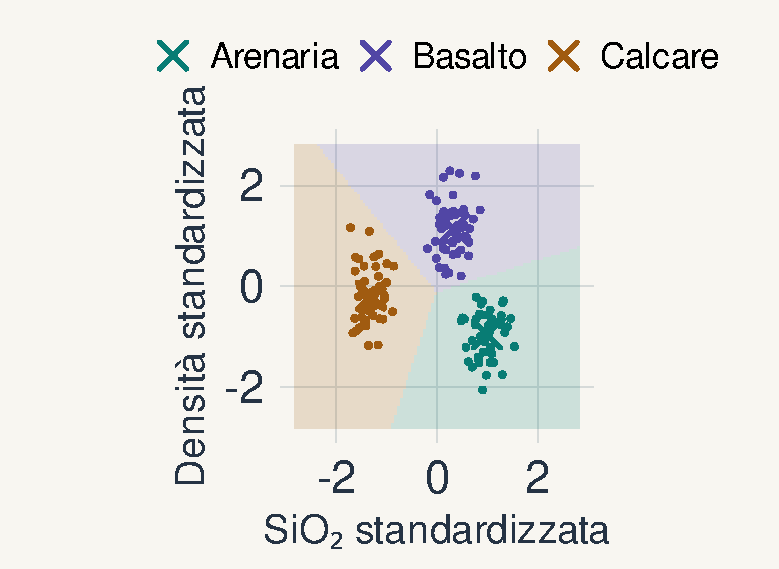
\includegraphics[width=\linewidth,height=6.15cm,keepaspectratio]{Figure/F05.pdf}\par}
\PSmall{z: punto nel piano standardizzato; $c_1,c_2$: due centroidi. L’equazione esprime uguale distanza; croci: centri stimati.}
}};
\node[anchor=north west,inner sep=0] at([xshift=10.85cm,yshift=-2.12cm]current page.north west){\Colonna{8.16cm}{\PBody{La figura adatta un classificatore distinto utilizzando soltanto silice e densità standardizzate, così da mostrare le regioni assegnate ai tre centroidi. Le frontiere separano punti equidistanti da due centri e risultano rette nella metrica euclidea. Le croci indicano i centroidi stimati, mentre i punti rappresentano l’addestramento. Questa vista illustra la geometria bidimensionale; le prestazioni riportate per il modello principale derivano invece dalle cinque variabili dichiarate e non possono essere lette direttamente da queste sole coordinate.}
\par\smallskip{\centering\adjustbox{max width=.98\linewidth}{$\displaystyle 2z^\top(c_2-c_1)=\|c_2\|^2-\|c_1\|^2$}\par\smallskip}
}};
\end{tikzpicture}\end{frame}

\begin{frame}[plain]\hypertarget{slide20}{}
\bookmark[level=1,page=20]{Vicini prossimi e voto locale}
\begin{tikzpicture}[remember picture,overlay]
\PilotChrome{Vicini prossimi e voto locale}{TRASFORMAZIONI E GEOMETRIA DELLA DECISIONE}{20}{Numero di vicini, scala e gestione dei pareggi definiscono insieme la regola di classificazione.}
\node[anchor=north west,inner sep=0] at([xshift=.96cm,yshift=-2.12cm]current page.north west){\Colonna{9.40cm}{{\centering\resizebox{.97\linewidth}{!}{\begin{tikzpicture}[x=1cm,y=-.87cm,every node/.style={font=\fontsize{12.2}{15}\selectfont,text=Ink},arr/.style={-{Stealth[length=2mm]},line width=.8pt,draw=Classical}]\path[use as bounding box] (0,0) rectangle (7.45,6.2);
\draw[Quantum,dashed,line width=.8pt] (3.7,3) ellipse [x radius=1.8cm,y radius=2.069cm];\fill[Measure] (3.7,3) circle (4pt);\fill[Classical] (2.5,2.5) circle (3pt);\fill[Classical] (3.2,1.5) circle (3pt);\fill[Quantum] (4.8,3.6) circle (3pt);\fill[Quantum] (5.8,1.5) circle (3pt);\fill[Classical] (1.2,4.8) circle (3pt);\node[anchor=center,text=Ink,font=\fontsize{11}{15}\selectfont,text width=6.7cm,align=center] at (3.7,0.4) {Tre vicini nella regione illustrata};
\node[anchor=center,text=Ink,font=\fontsize{11}{15}\selectfont,text width=6.8cm,align=center] at (3.7,5.8) {Il voto dipende da distanza e numero di vicini.};

\end{tikzpicture}}\par}
\PSmall{$N_k(z)$: indici dei vicini, compresi gli eventuali ex aequo sulla distanza; $y_i$: classe del vicino. Si contano i voti per ogni classe c.}
}};
\node[anchor=north west,inner sep=0] at([xshift=10.85cm,yshift=-2.12cm]current page.north west){\Colonna{8.16cm}{\PBody{Il metodo dei k vicini assegna la classe mediante il voto dei campioni più prossimi nella metrica prescelta. Un valore piccolo di k descrive variazioni locali fini, mentre un valore maggiore amplia il vicinato e modifica il compromesso fra flessibilità e stabilità. Le regole sui pareggi possono incidere sul risultato: class::knn include per impostazione predefinita le distanze pari a quella del k-esimo vicino e risolve casualmente i pareggi di voto. Seme e convenzioni vengono pertanto registrati nel codice.}
\par\smallskip{\centering\adjustbox{max width=.98\linewidth}{$\displaystyle \widehat y(z)=\arg\max_c\sum_{i\in N_k(z)}\mathbf1\{y_i=c\}$}\par\smallskip}
}};
\end{tikzpicture}\end{frame}

\begin{frame}[plain]\hypertarget{slide21}{}
\bookmark[level=1,page=21]{Il test conserva lo scarto dal centro del training}
\begin{tikzpicture}[remember picture,overlay]
\PilotChrome{Il test conserva lo scarto dal centro del training}{TRASFORMAZIONI E GEOMETRIA DELLA DECISIONE}{21}{Centro e scala sono stimati nel training e applicati al test.}
\node[anchor=north west,inner sep=0] at([xshift=.96cm,yshift=-2.12cm]current page.north west){\Colonna{9.40cm}{\PLabel{Risultati del calcolo in R}
{\fontsize{10.2}{12.8}\selectfont\begin{tabular}{@{}>{\raggedright\arraybackslash}p{0.22\linewidth}@{\hspace{.13cm}}>{\raggedright\arraybackslash}p{0.22\linewidth}@{\hspace{.13cm}}>{\raggedright\arraybackslash}p{0.22\linewidth}@{\hspace{.13cm}}>{\raggedright\arraybackslash}p{0.23\linewidth}@{}}\toprule variabile & media train & sd train & media test\\[2.3pt]
\midrule 
SiO2 & -2,43e-17 & 1 & -0,097284\\[2.3pt]
CaO & 3,81e-17 & 1 & 0,0041041\\[2.3pt]
MgO & 1,66e-17 & 1 & -0,12761\\[2.3pt]
FeO & -6,60e-17 & 1 & 0,0024835\\[2.3pt]
densita & 1,09e-15 & 1 & 0,020751\\[2.3pt]
\bottomrule\end{tabular}\par}
}};
\node[anchor=north west,inner sep=0] at([xshift=10.85cm,yshift=-2.12cm]current page.north west){\Colonna{8.16cm}{\PBody{Perché la media dei predittori standardizzati nel test può essere diversa da zero?}
\vspace{.4cm}\PInfo{Centro e scala sono stimati nel training e applicati al test. Ricentrare separatamente il test cambierebbe il sistema di misura usato dal classificatore.}
}};
\node[anchor=north east,inner sep=0] at([xshift=17.1cm,yshift=-12.04cm]current page.north west){\fontsize{7.7}{9}\selectfont \href{https://github.com/marzione00/Lab_Geo/blob/649f7cc577b96bd1044d81e78a2f530813e4f96b/materiali/laboratori/M16/M16_N04.R}{\color{Classical}\bfseries Script R · M16\_N04}};
\end{tikzpicture}\end{frame}

\begin{frame}[plain]\hypertarget{slide22}{}
\bookmark[level=1,page=22]{Il centroide assegna una classe a ogni provino}
\begin{tikzpicture}[remember picture,overlay]
\PilotChrome{Il centroide assegna una classe a ogni provino}{TRASFORMAZIONI E GEOMETRIA DELLA DECISIONE}{22}{Conserva ID, classe osservata e classe prevista insieme.}
\node[anchor=north west,inner sep=0] at([xshift=.96cm,yshift=-2.12cm]current page.north west){\Colonna{9.40cm}{\PLabel{Risultati del calcolo in R}
{\fontsize{10.2}{12.8}\selectfont\begin{tabular}{@{}>{\raggedright\arraybackslash}p{0.22\linewidth}@{\hspace{.13cm}}>{\raggedright\arraybackslash}p{0.22\linewidth}@{\hspace{.13cm}}>{\raggedright\arraybackslash}p{0.22\linewidth}@{\hspace{.13cm}}>{\raggedright\arraybackslash}p{0.23\linewidth}@{}}\toprule id & osservata & prevista & corretta\\[2.3pt]
\midrule 
R051 & Basalto & Basalto & sì\\[2.3pt]
R052 & Basalto & Basalto & sì\\[2.3pt]
R116 & Arenaria & Arenaria & sì\\[2.3pt]
R179 & Calcare & Calcare & sì\\[2.3pt]
R180 & Calcare & Calcare & sì\\[2.3pt]
\bottomrule\end{tabular}\par}
\PSmall{Selezione di cinque righe dal file completo.}
}};
\node[anchor=north west,inner sep=0] at([xshift=10.85cm,yshift=-2.12cm]current page.north west){\Colonna{8.16cm}{\PBody{Quali informazioni servono per controllare un singolo errore di classificazione?}
\vspace{.4cm}\PInfo{Conserva ID, classe osservata e classe prevista insieme. Una percentuale aggregata perde la possibilità di localizzare errori per stazione o litologia.}
}};
\node[anchor=north east,inner sep=0] at([xshift=17.1cm,yshift=-12.04cm]current page.north west){\fontsize{7.7}{9}\selectfont \href{https://github.com/marzione00/Lab_Geo/blob/649f7cc577b96bd1044d81e78a2f530813e4f96b/materiali/laboratori/M16/M16_N05.R}{\color{Classical}\bfseries Script R · M16\_N05}};
\end{tikzpicture}\end{frame}

\begin{frame}[plain]\hypertarget{slide23}{}
\bookmark[level=1,page=23]{Standardizzazione e confine decisionale}
\begin{tikzpicture}[remember picture,overlay]
\PilotChrome{Standardizzazione e confine decisionale}{TRASFORMAZIONI E GEOMETRIA DELLA DECISIONE}{23}{Esaminare un classificatore a centroidi nella metrica scelta.}
\node[anchor=north west,inner sep=0] at([xshift=.96cm,yshift=-2.12cm]current page.north west){\Colonna{9.40cm}{{\centering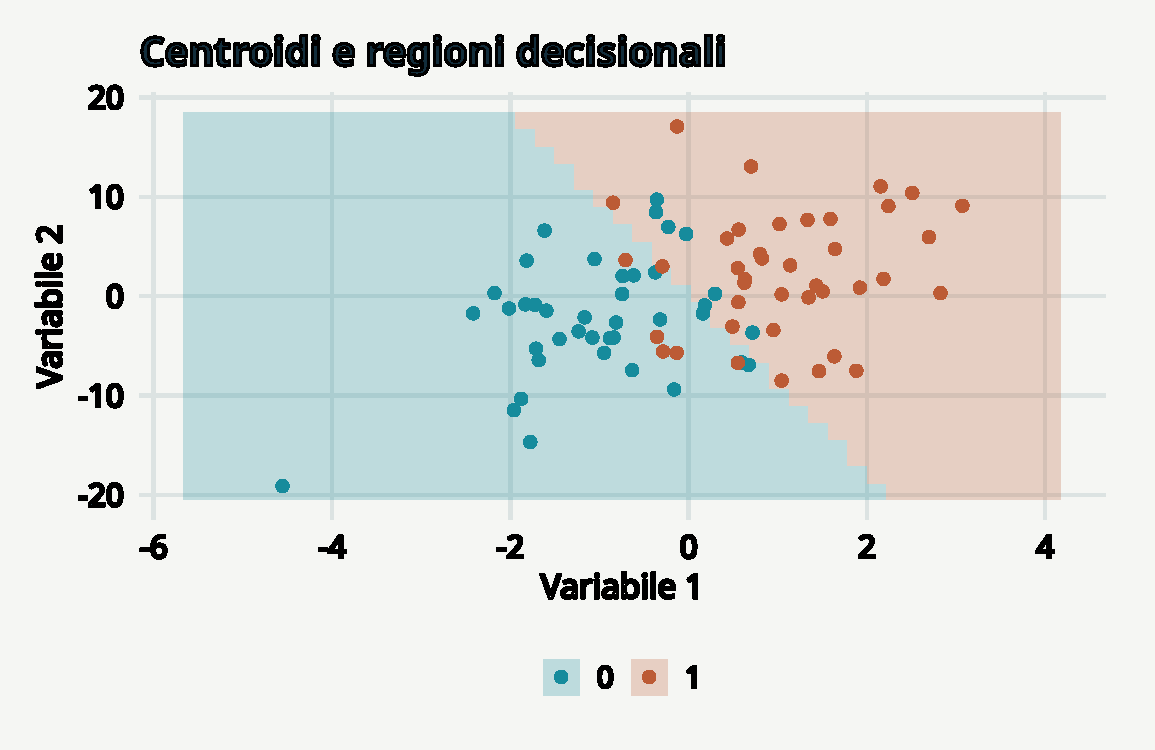
\includegraphics[width=\linewidth,height=6.0cm,keepaspectratio]{Esperimenti/m16-geometria-A.pdf}\par}
\PSmall{Standardizzazione: Sì. Seme: 17.}
}};
\node[anchor=north west,inner sep=0] at([xshift=10.85cm,yshift=-2.12cm]current page.north west){\Colonna{8.16cm}{\PLabel{Scenario A · simulazione}
\PBody{Un classificatore a centroidi assegna una nuova osservazione al gruppo il cui centro è più vicino nella metrica adottata. Il campione sintetico contiene due classi e due variabili; il controllo moltiplica la seconda variabile, mentre la standardizzazione ne può compensare il cambiamento di scala. Le regioni colorate mostrano la decisione ottenuta in ciascuna posizione.}
\par\smallskip{\centering\adjustbox{max width=.98\linewidth}{$\displaystyle \widehat c(x)=\arg\min_k\lVert T(x)-\mu_k\rVert^2$}\par\smallskip}
\PSmall{T(x) è il vettore dopo la trasformazione scelta, $\mu_k$ il centroide della classe k e $\hat c(x)$ la classe assegnata. La norma quadratica misura la distanza nello spazio trasformato; in caso di parità il codice assegna la classe zero.}
}};
\node[anchor=north east,inner sep=0] at([xshift=17.1cm,yshift=-12.04cm]current page.north west){\fontsize{7.7}{9}\selectfont \href{https://marzione00.github.io/Lab_Geo/\#laboratorio/m16-geometria}{\color{Classical}\bfseries Apri il laboratorio · m16-geometria}};
\end{tikzpicture}\end{frame}

\begin{frame}[plain]\hypertarget{slide24}{}
\bookmark[level=1,page=24]{Confronto | Standardizzazione e confine decisionale}
\begin{tikzpicture}[remember picture,overlay]
\PilotChrome{Confronto | Standardizzazione e confine decisionale}{TRASFORMAZIONI E GEOMETRIA DELLA DECISIONE}{24}{La distanza utilizzata dal classificatore dipende dalla trasformazione stimata sul campione di addestramento.}
\node[anchor=north west,inner sep=0] at([xshift=.96cm,yshift=-2.12cm]current page.north west){\Colonna{9.40cm}{{\centering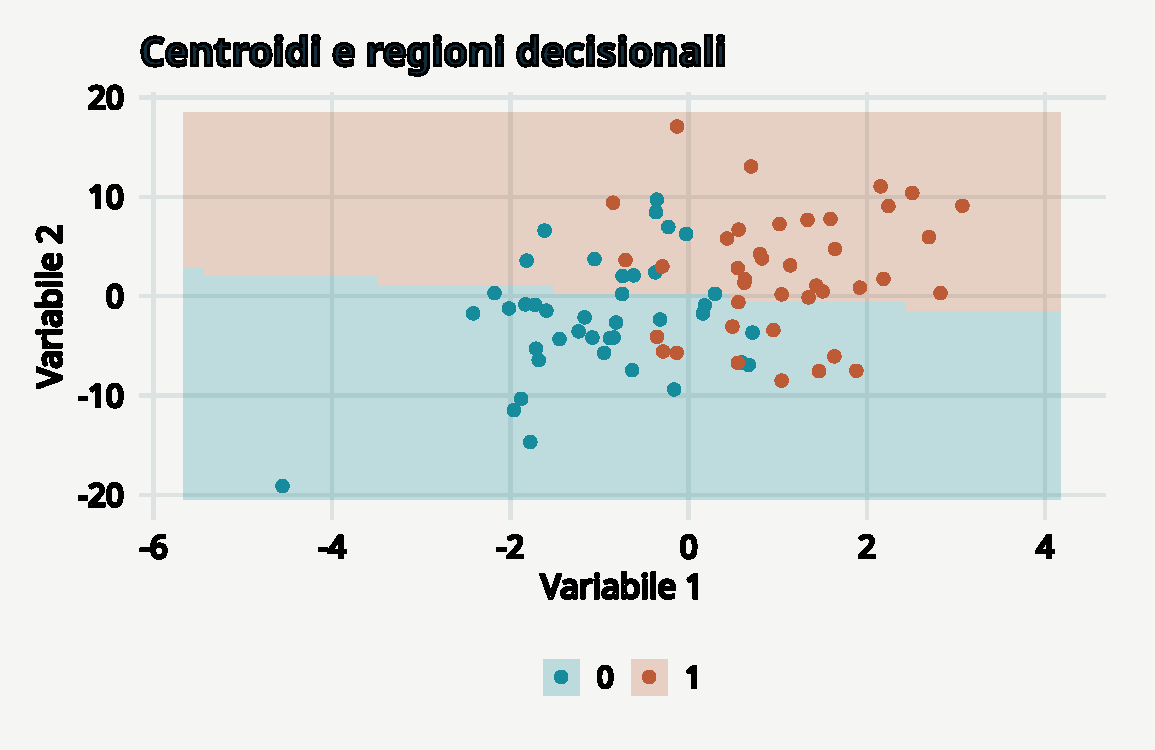
\includegraphics[width=\linewidth,height=5.6cm,keepaspectratio]{Esperimenti/m16-geometria-B.pdf}\par}
\PSmall{Standardizzazione: Sì $\to$ No. Tutti gli altri parametri e il seme sono fissi.}
}};
\node[anchor=north west,inner sep=0] at([xshift=10.85cm,yshift=-2.12cm]current page.north west){\Colonna{8.16cm}{\PLabel{Confronto fra gli scenari}
{\fontsize{10.2}{12.8}\selectfont\begin{tabular}{@{}>{\raggedright\arraybackslash}p{0.48\linewidth}@{\hspace{.13cm}}>{\raggedright\arraybackslash}p{0.224\linewidth}@{\hspace{.13cm}}>{\raggedright\arraybackslash}p{0.224\linewidth}@{}}\toprule Grandezza & A & B\\[2.3pt]
\midrule 
Scala applicata a X2 & 5 & 5\\[2.3pt]
SD usata per X2 & 6,49 & 1\\[2.3pt]
\bottomrule\end{tabular}\par}
\vspace{.25cm}\PBody{Disattivare la standardizzazione cambia la geometria delle distanze. La scala viene mantenuta fissa fra i due confronti per isolare questo effetto.}
}};
\node[anchor=north east,inner sep=0] at([xshift=17.1cm,yshift=-12.04cm]current page.north west){\fontsize{7.7}{9}\selectfont \href{https://marzione00.github.io/Lab_Geo/\#laboratorio/m16-geometria}{\color{Classical}\bfseries Apri il laboratorio · m16-geometria}};
\end{tikzpicture}\end{frame}

\begin{frame}[plain]\hypertarget{slide25}{}
\bookmark[level=0,page=25]{Selezione e validazione per gruppi}
\bookmark[level=1,page=25]{Una stazione esclusa resta fuori dalla selezione}
\begin{tikzpicture}[remember picture,overlay]
\PilotChrome{Una stazione esclusa resta fuori dalla selezione}{SELEZIONE E VALIDAZIONE PER GRUPPI}{25}{Fissa metrica, partizioni e criterio di pareggio prima di interrogare il test.}
\node[anchor=north west,inner sep=0] at([xshift=.96cm,yshift=-2.12cm]current page.north west){\Colonna{9.40cm}{\PLabel{Domanda}
\PBody{Tre candidati k vengono valutati su partizioni interne del training. Due raggiungono lo stesso punteggio medio. Quale regola rende ripetibile la scelta?}
\vspace{.35cm}\PLabel{Interpretazione}
\PBody{Applicando la regola dichiarata “scegli il k minore a parità di punteggio” si seleziona 3. Il test esterno può essere aperto dopo questa scelta.}
}};
\node[anchor=north west,inner sep=0] at([xshift=10.85cm,yshift=-2.12cm]current page.north west){\Colonna{8.16cm}{\begin{tcolorbox}[enhanced,arc=1.7mm,boxrule=.6pt,colback=white,colframe=Classical!60!Navy,colbacktitle=Navy,coltitle=white,fonttitle=\bfseries\small,title={R · calcolo riproducibile},left=1.7mm,right=1.3mm,top=1.1mm,bottom=1.1mm,before skip=1mm,after skip=1.0mm]\lstinputlisting[style=GeoR,language=R]{Codice/capitolo-03.R}\end{tcolorbox}
\PLabel{Risultato in R}
\begin{tcolorbox}[colback=GeoTint,colframe=Rule,boxrule=.5pt,arc=1.4mm,left=2mm,right=1mm,top=1mm,bottom=1mm]{\fontsize{9}{12}\selectfont\ttfamily \mbox{[1]\ 3}}\end{tcolorbox}}};
\end{tikzpicture}\end{frame}

\begin{frame}[plain]\hypertarget{slide26}{}
\bookmark[level=1,page=26]{Ogni partizione ripete l’intera procedura}
\begin{tikzpicture}[remember picture,overlay]
\PilotChrome{Ogni partizione ripete l’intera procedura}{SELEZIONE E VALIDAZIONE PER GRUPPI}{26}{La validazione valuta una procedura completa, comprese le trasformazioni stimate dai dati.}
\node[anchor=north west,inner sep=0] at([xshift=.96cm,yshift=-2.12cm]current page.north west){\Colonna{9.40cm}{{\centering\resizebox{.97\linewidth}{!}{\begin{tikzpicture}[x=1cm,y=-.87cm,every node/.style={font=\fontsize{12.2}{15}\selectfont,text=Ink},arr/.style={-{Stealth[length=2mm]},line width=.8pt,draw=Classical}]\path[use as bounding box] (0,0) rectangle (7.45,6.2);
\draw[draw=Classical,fill=Classical!8,rounded corners=2pt,line width=.7pt] (0.5,0.4) rectangle (6.9,1.5499999999999998);
\node[anchor=center,text=Ink,font=\fontsize{11.5}{15}\selectfont,text width=6cm,align=center] at (3.7,0.975) {12 stazioni: trasformazione e adattamento};
\draw[arr,draw=Classical] (3.7,1.7000000000000002)--(3.7,2.08);
\draw[draw=Quantum,fill=Quantum!8,rounded corners=2pt,line width=.7pt] (0.5,2.25) rectangle (6.9,3.4);
\node[anchor=center,text=Ink,font=\fontsize{11.5}{15}\selectfont,text width=6cm,align=center] at (3.7,2.825) {3 stazioni: previsione e perdita};
\draw[arr,draw=Classical] (3.7,3.55)--(3.7,3.9299999999999997);
\draw[draw=Classical,fill=Classical!8,rounded corners=2pt,line width=.7pt] (0.5,4.1000000000000005) rectangle (6.9,5.25);
\node[anchor=center,text=Ink,font=\fontsize{11.5}{15}\selectfont,text width=6cm,align=center] at (3.7,4.675000000000001) {Ripetizione per cinque partizioni};

\end{tikzpicture}}\par}
}};
\node[anchor=north west,inner sep=0] at([xshift=10.85cm,yshift=-2.12cm]current page.north west){\Colonna{8.16cm}{\PBody{La validazione interna divide le quindici stazioni di addestramento in cinque partizioni, ciascuna delle quali esclude una stazione per classe. In ogni passaggio si ristimano media e deviazione standard sulle dodici stazioni rimaste, si adatta il classificatore e si predicono le tre stazioni escluse. Il test esterno resta fuori da queste operazioni. Calcolare la standardizzazione una sola volta su tutto l’addestramento trasferirebbe nel modello informazioni della partizione che dovrebbe essere esclusa.}
}};
\end{tikzpicture}\end{frame}

\begin{frame}[plain]\hypertarget{slide27}{}
\bookmark[level=1,page=27]{Selezione di k e regola per i pareggi}
\begin{tikzpicture}[remember picture,overlay]
\PilotChrome{Selezione di k e regola per i pareggi}{SELEZIONE E VALIDAZIONE PER GRUPPI}{27}{L’uguaglianza delle prestazioni limita le conclusioni comparative consentite dal dataset.}
\node[anchor=north west,inner sep=0] at([xshift=.96cm,yshift=-2.12cm]current page.north west){\Colonna{9.40cm}{{\centering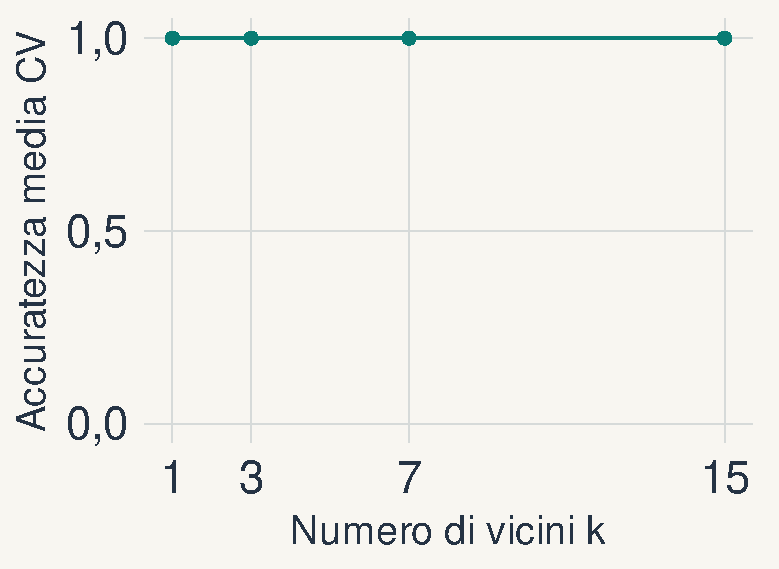
\includegraphics[width=\linewidth,height=6.15cm,keepaspectratio]{Figure/F03.pdf}\par}
\PSmall{$Acc_v(k)$: frazione corretta nella partizione esclusa v. Tutti i valori sono 1; il pareggio prestabilito seleziona k = 1.}
}};
\node[anchor=north west,inner sep=0] at([xshift=10.85cm,yshift=-2.12cm]current page.north west){\Colonna{8.16cm}{\PBody{I valori uno, tre, sette e quindici vengono confrontati sulle stesse cinque partizioni per stazioni. In questo dataset tutti ottengono accuratezza media pari a uno, per cui la regola prestabilita seleziona il primo valore della lista. Il pareggio rivela che l’esempio distingue poco le alternative e impedisce di attribuire superiorità sostanziale al valore scelto. Le prestazioni utilizzate per selezionare un parametro restano risultati di selezione; una valutazione conclusiva richiede dati esterni al processo decisionale oppure una validazione annidata.}
\par\smallskip{\centering\adjustbox{max width=.98\linewidth}{$\displaystyle \widehat k=\arg\max_{k\in\{1,3,7,15\}}\frac15\sum_{v=1}^{5}Acc_v(k)$}\par\smallskip}
}};
\end{tikzpicture}\end{frame}

\begin{frame}[plain]\hypertarget{slide28}{}
\bookmark[level=1,page=28]{Separare esplorazione e valutazione conclusiva}
\begin{tikzpicture}[remember picture,overlay]
\PilotChrome{Separare esplorazione e valutazione conclusiva}{SELEZIONE E VALIDAZIONE PER GRUPPI}{28}{La storia delle decisioni determina il ruolo effettivo dei dati nella valutazione.}
\node[anchor=north west,inner sep=0] at([xshift=.96cm,yshift=-2.12cm]current page.north west){\Colonna{9.40cm}{{\centering\resizebox{.97\linewidth}{!}{\begin{tikzpicture}[x=1cm,y=-.87cm,every node/.style={font=\fontsize{12.2}{15}\selectfont,text=Ink},arr/.style={-{Stealth[length=2mm]},line width=.8pt,draw=Classical}]\path[use as bounding box] (0,0) rectangle (7.45,6.2);
\draw[draw=Classical,fill=Classical!8,rounded corners=2pt,line width=.7pt] (0.5,0.4) rectangle (6.9,1.6);
\node[anchor=center,text=Ink,font=\fontsize{12.2}{15}\selectfont,text width=6cm,align=center] at (3.7,1) {Sviluppo e selezione interna};
\draw[arr,draw=Classical] (3.7,1.8)--(3.7,2.4);
\draw[Measure,line width=.8pt] (0.5,2.7)--(6.9,2.7);
\node[anchor=center,text=Measure,font=\fontsize{12.2}{15}\selectfont,text width=6cm,align=center] at (3.7,3.2) {Scelte fissate};
\draw[arr,draw=Classical] (3.7,3.7)--(3.7,4.3);
\draw[draw=Quantum,fill=Quantum!8,rounded corners=2pt,line width=.7pt] (0.5,4.5) rectangle (6.9,5.7);
\node[anchor=center,text=Ink,font=\fontsize{12.2}{15}\selectfont,text width=6cm,align=center] at (3.7,5.1) {Valutazione su dati ulteriori};

\end{tikzpicture}}\par}
}};
\node[anchor=north west,inner sep=0] at([xshift=10.85cm,yshift=-2.12cm]current page.north west){\Colonna{8.16cm}{\PBody{Le esercitazioni confrontano più metodi e riutilizzano le etichette di test per chiarirne il funzionamento. Il loro insieme costituisce un percorso didattico esplorativo, del quale sarebbe improprio presentare il migliore risultato come valutazione finale indipendente. In un progetto applicato, scelte di variabili, trasformazioni, parametri e soglie vengono fissate prima di consultare il test conclusivo. Se i risultati del test inducono nuove modifiche, quella porzione di dati entra nel processo di sviluppo e occorre una verifica ulteriore.}
}};
\end{tikzpicture}\end{frame}

\begin{frame}[plain]\hypertarget{slide29}{}
\bookmark[level=1,page=29]{La verifica interna valuta stazioni escluse}
\begin{tikzpicture}[remember picture,overlay]
\PilotChrome{La verifica interna valuta stazioni escluse}{SELEZIONE E VALIDAZIONE PER GRUPPI}{29}{In questo dataset sintetico i gruppi sono fortemente separati.}
\node[anchor=north west,inner sep=0] at([xshift=.96cm,yshift=-2.12cm]current page.north west){\Colonna{9.40cm}{\PLabel{Risultati del calcolo in R}
{\fontsize{10.2}{12.8}\selectfont\begin{tabular}{@{}>{\raggedright\arraybackslash}p{0.44\linewidth}@{\hspace{.13cm}}>{\raggedright\arraybackslash}p{0.48\linewidth}@{}}\toprule fold & Accuratezza\\[2.3pt]
\midrule 
1 & 1\\[2.3pt]
2 & 1\\[2.3pt]
3 & 1\\[2.3pt]
4 & 1\\[2.3pt]
5 & 1\\[2.3pt]
\bottomrule\end{tabular}\par}
}};
\node[anchor=north west,inner sep=0] at([xshift=10.85cm,yshift=-2.12cm]current page.north west){\Colonna{8.16cm}{\PBody{La precisione elevata si ripete attraverso le cinque partizioni?}
\vspace{.4cm}\PInfo{In questo dataset sintetico i gruppi sono fortemente separati. Un punteggio uniforme nelle partizioni richiede comunque una verifica su stazioni davvero nuove.}
}};
\node[anchor=north east,inner sep=0] at([xshift=17.1cm,yshift=-12.04cm]current page.north west){\fontsize{7.7}{9}\selectfont \href{https://github.com/marzione00/Lab_Geo/blob/649f7cc577b96bd1044d81e78a2f530813e4f96b/materiali/laboratori/M16/M16_N10.R}{\color{Classical}\bfseries Script R · M16\_N10}};
\end{tikzpicture}\end{frame}

\begin{frame}[plain]\hypertarget{slide30}{}
\bookmark[level=1,page=30]{Più valori di k possono ottenere lo stesso punteggio}
\begin{tikzpicture}[remember picture,overlay]
\PilotChrome{Più valori di k possono ottenere lo stesso punteggio}{SELEZIONE E VALIDAZIONE PER GRUPPI}{30}{Tutti i candidati qui raggiungono la stessa accuratezza interna.}
\node[anchor=north west,inner sep=0] at([xshift=.96cm,yshift=-2.12cm]current page.north west){\Colonna{9.40cm}{\PLabel{Risultati del calcolo in R}
{\fontsize{10.2}{12.8}\selectfont\begin{tabular}{@{}>{\raggedright\arraybackslash}p{0.44\linewidth}@{\hspace{.13cm}}>{\raggedright\arraybackslash}p{0.48\linewidth}@{}}\toprule k & Acc. interna\\[2.3pt]
\midrule 
1 & 1\\[2.3pt]
3 & 1\\[2.3pt]
7 & 1\\[2.3pt]
15 & 1\\[2.3pt]
\bottomrule\end{tabular}\par}
}};
\node[anchor=north west,inner sep=0] at([xshift=10.85cm,yshift=-2.12cm]current page.north west){\Colonna{8.16cm}{\PBody{Il dato discrimina fra i numeri di vicini candidati?}
\vspace{.4cm}\PInfo{Tutti i candidati qui raggiungono la stessa accuratezza interna. La scelta dipende quindi dalla regola di pareggio dichiarata.}
}};
\node[anchor=north east,inner sep=0] at([xshift=17.1cm,yshift=-12.04cm]current page.north west){\fontsize{7.7}{9}\selectfont \href{https://github.com/marzione00/Lab_Geo/blob/649f7cc577b96bd1044d81e78a2f530813e4f96b/materiali/laboratori/M16/M16_N11.R}{\color{Classical}\bfseries Script R · M16\_N11}};
\end{tikzpicture}\end{frame}

\begin{frame}[plain]\hypertarget{slide31}{}
\bookmark[level=1,page=31]{Selezione dei predittori e contaminazione}
\begin{tikzpicture}[remember picture,overlay]
\PilotChrome{Selezione dei predittori e contaminazione}{SELEZIONE E VALIDAZIONE PER GRUPPI}{31}{Valutare la selezione di variabili su puro rumore.}
\node[anchor=north west,inner sep=0] at([xshift=.96cm,yshift=-2.12cm]current page.north west){\Colonna{9.40cm}{{\centering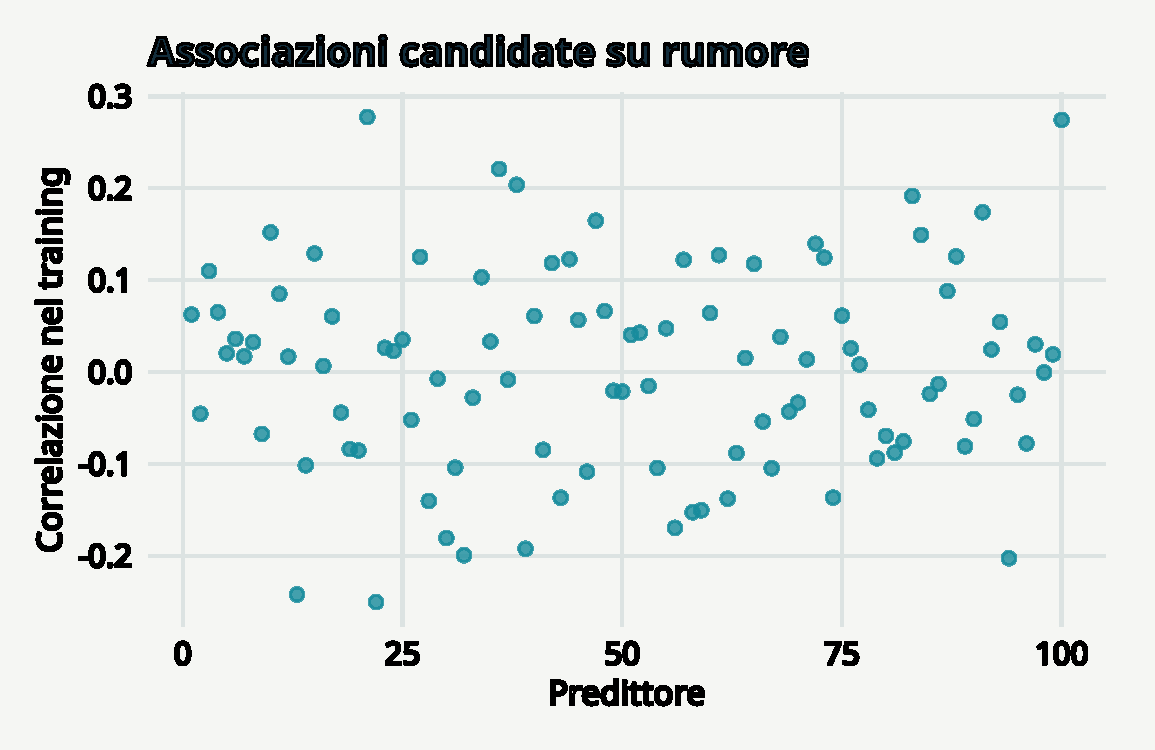
\includegraphics[width=\linewidth,height=6.0cm,keepaspectratio]{Esperimenti/m16-selezione-A.pdf}\par}
\PSmall{Predittori candidati: 100. Seme: 17.}
}};
\node[anchor=north west,inner sep=0] at([xshift=10.85cm,yshift=-2.12cm]current page.north west){\Colonna{8.16cm}{\PLabel{Scenario A · simulazione}
\PBody{La ricerca fra molti predittori può individuare associazioni apparenti anche quando tutte le variabili sono indipendenti dal bersaglio. Nell’esperimento si sceglie il predittore con massima correlazione assoluta, confrontando una selezione eseguita soltanto sul campione di addestramento con una che utilizza anche le risposte del test. Entrambi i modelli vengono poi adattati sul medesimo training.}
\par\smallskip{\centering\adjustbox{max width=.98\linewidth}{$\displaystyle j^*=\arg\max_j|\operatorname{cor}(X_j,Y)|$}\par\smallskip}
\PSmall{$X_j$ è il predittore candidato j, Y la risposta binaria e $j^*$ l’indice selezionato. Il criterio massimizza il valore assoluto della correlazione campionaria, che viene calcolata su insiemi diversi nei due protocolli.}
}};
\node[anchor=north east,inner sep=0] at([xshift=17.1cm,yshift=-12.04cm]current page.north west){\fontsize{7.7}{9}\selectfont \href{https://marzione00.github.io/Lab_Geo/\#laboratorio/m16-selezione}{\color{Classical}\bfseries Apri il laboratorio · m16-selezione}};
\end{tikzpicture}\end{frame}

\begin{frame}[plain]\hypertarget{slide32}{}
\bookmark[level=1,page=32]{Confronto | Selezione dei predittori e contaminazione}
\begin{tikzpicture}[remember picture,overlay]
\PilotChrome{Confronto | Selezione dei predittori e contaminazione}{SELEZIONE E VALIDAZIONE PER GRUPPI}{32}{La selezione informata dal test compromette l’indipendenza della valutazione.}
\node[anchor=north west,inner sep=0] at([xshift=.96cm,yshift=-2.12cm]current page.north west){\Colonna{9.40cm}{{\centering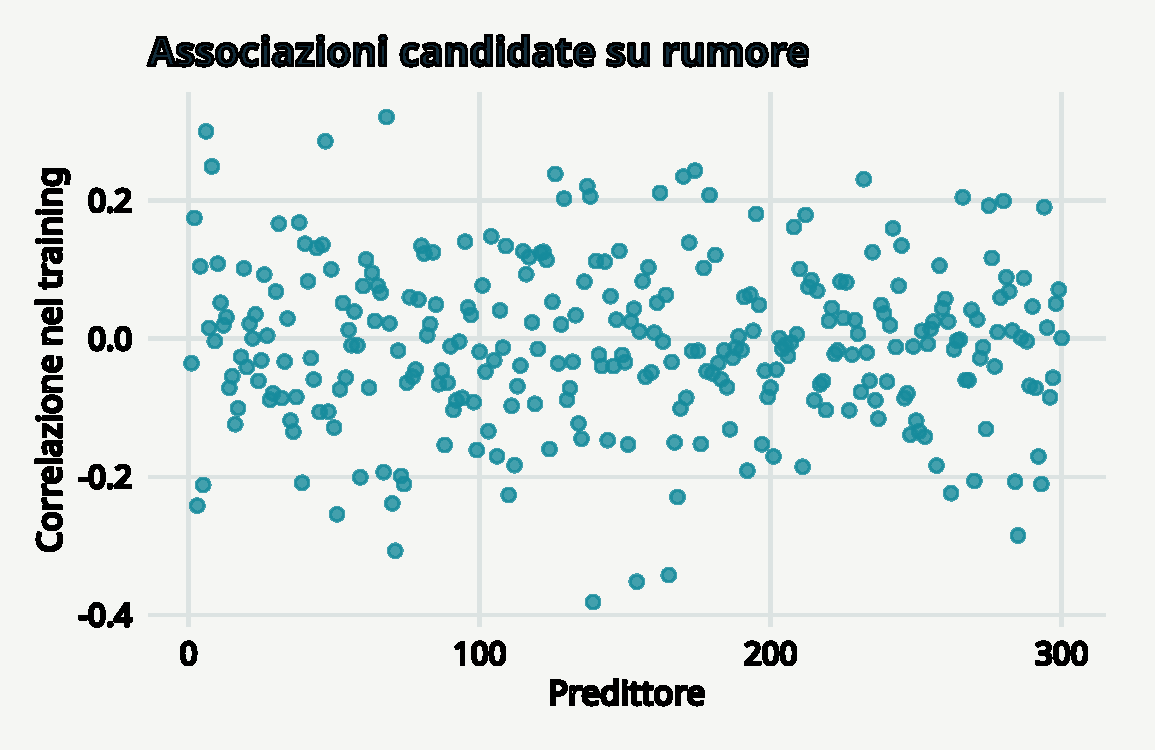
\includegraphics[width=\linewidth,height=5.6cm,keepaspectratio]{Esperimenti/m16-selezione-B.pdf}\par}
\PSmall{Predittori candidati: 100 $\to$ 300. Tutti gli altri parametri e il seme sono fissi.}
}};
\node[anchor=north west,inner sep=0] at([xshift=10.85cm,yshift=-2.12cm]current page.north west){\Colonna{8.16cm}{\PLabel{Confronto fra gli scenari}
{\fontsize{10.2}{12.8}\selectfont\begin{tabular}{@{}>{\raggedright\arraybackslash}p{0.48\linewidth}@{\hspace{.13cm}}>{\raggedright\arraybackslash}p{0.224\linewidth}@{\hspace{.13cm}}>{\raggedright\arraybackslash}p{0.224\linewidth}@{}}\toprule Grandezza & A & B\\[2.3pt]
\midrule 
Accuratezza selezione sul training & 0,45 & 0,375\\[2.3pt]
Accuratezza selezione contaminata & 0,575 & 0,65\\[2.3pt]
Massima correlazione assoluta training & 0,277 & 0,381\\[2.3pt]
\bottomrule\end{tabular}\par}
\vspace{.25cm}\PBody{Con più candidati cresce l’opportunità di trovare associazioni casuali. La selezione contaminata dal test appare più favorevole in questo campione.}
}};
\node[anchor=north east,inner sep=0] at([xshift=17.1cm,yshift=-12.04cm]current page.north west){\fontsize{7.7}{9}\selectfont \href{https://marzione00.github.io/Lab_Geo/\#laboratorio/m16-selezione}{\color{Classical}\bfseries Apri il laboratorio · m16-selezione}};
\end{tikzpicture}\end{frame}

\begin{frame}[plain]\hypertarget{slide33}{}
\bookmark[level=0,page=33]{Alberi e insiemi di classificatori}
\bookmark[level=1,page=33]{Una divisione può rendere i figli più omogenei}
\begin{tikzpicture}[remember picture,overlay]
\PilotChrome{Una divisione può rendere i figli più omogenei}{ALBERI E INSIEMI DI CLASSIFICATORI}{33}{La riduzione dell’impurità misura il miglioramento locale sui dati di addestramento.}
\node[anchor=north west,inner sep=0] at([xshift=.96cm,yshift=-2.12cm]current page.north west){\Colonna{9.40cm}{\PLabel{Domanda}
\PBody{Un nodo contiene quattro basalti e quattro arenarie. Una divisione crea due figli con proporzioni 3:1 e 1:3. Quanto cambia l’impurità media?}
\vspace{.35cm}\PLabel{Interpretazione}
\PBody{L’impurità scende da 0,5 a 0,375 nel training. Per sapere se la regola si trasferisce occorre provarla su stazioni escluse.}
}};
\node[anchor=north west,inner sep=0] at([xshift=10.85cm,yshift=-2.12cm]current page.north west){\Colonna{8.16cm}{\begin{tcolorbox}[enhanced,arc=1.7mm,boxrule=.6pt,colback=white,colframe=Classical!60!Navy,colbacktitle=Navy,coltitle=white,fonttitle=\bfseries\small,title={R · calcolo riproducibile},left=1.7mm,right=1.3mm,top=1.1mm,bottom=1.1mm,before skip=1mm,after skip=1.0mm]\lstinputlisting[style=GeoR,language=R]{Codice/capitolo-04.R}\end{tcolorbox}
\PLabel{Risultato in R}
\begin{tcolorbox}[colback=GeoTint,colframe=Rule,boxrule=.5pt,arc=1.4mm,left=2mm,right=1mm,top=1mm,bottom=1mm]{\fontsize{9}{12}\selectfont\ttfamily \mbox{prima\ \ \ \ \ \ dopo\ riduzione\ }\\\mbox{\ \ \ \ 0.500\ \ \ \ \ 0.375\ \ \ \ \ 0.125}}\end{tcolorbox}}};
\end{tikzpicture}\end{frame}

\begin{frame}[plain]\hypertarget{slide34}{}
\bookmark[level=1,page=34]{Partizioni ricorsive e impurità di un nodo}
\begin{tikzpicture}[remember picture,overlay]
\PilotChrome{Partizioni ricorsive e impurità di un nodo}{ALBERI E INSIEMI DI CLASSIFICATORI}{34}{Una soglia appresa descrive la partizione del modello entro il campione e il protocollo utilizzati.}
\node[anchor=north west,inner sep=0] at([xshift=.96cm,yshift=-2.12cm]current page.north west){\Colonna{9.40cm}{{\centering\resizebox{.97\linewidth}{!}{\begin{tikzpicture}[x=1cm,y=-.87cm,every node/.style={font=\fontsize{12.2}{15}\selectfont,text=Ink},arr/.style={-{Stealth[length=2mm]},line width=.8pt,draw=Classical}]\path[use as bounding box] (0,0) rectangle (7.45,6.2);
\draw[draw=Classical,fill=Classical!8,rounded corners=2pt,line width=.7pt] (1.8,0.4) rectangle (5.6,1.6);
\node[anchor=center,text=Ink,font=\fontsize{17}{15}\selectfont] at (3.7,1) {$x_j\leq c$};
\draw[arr,draw=Classical] (2.7,1.8)--(1.8,3);
\draw[arr,draw=Quantum] (4.7,1.8)--(5.6,3);
\draw[draw=Classical,fill=Classical!8,rounded corners=2pt,line width=.7pt] (0.5,3.2) rectangle (3.2,4.7);
\draw[draw=Quantum,fill=Quantum!8,rounded corners=2pt,line width=.7pt] (4.2,3.2) rectangle (6.9,4.7);
\node[anchor=center,text=Ink,font=\fontsize{12.2}{15}\selectfont,text width=2.3cm,align=center] at (1.85,3.95) {Nodo L};
\node[anchor=center,text=Ink,font=\fontsize{12.2}{15}\selectfont,text width=2.3cm,align=center] at (5.55,3.95) {Nodo R};
\node[anchor=center,text=Ink,font=\fontsize{11}{15}\selectfont,text width=6.5cm,align=center] at (3.7,5.6) {Soglia appresa, unità originali.};

\end{tikzpicture}}\par}
\PSmall{$p_{c|t}$: quota della classe c nel nodo t; $n_t$: numerosità. L e R sono i figli, con $n_L+n_R=n_t$.}
}};
\node[anchor=north west,inner sep=0] at([xshift=10.85cm,yshift=-2.12cm]current page.north west){\Colonna{8.16cm}{\PBody{Un albero suddivide lo spazio dei predittori mediante condizioni successive e assegna una classe nelle regioni terminali. L’impurità di Gini misura la mescolanza delle classi in un nodo; una separazione viene valutata attraverso la riduzione dell’impurità, ponderando i nodi figli per la loro numerosità. Le soglie apprese mantengono le unità originali. Nel laboratorio la profondità massima è tre, con parametri di crescita espliciti e senza attribuire alle soglie una validità petrografica universale.}
\par\smallskip{\centering\adjustbox{max width=.98\linewidth}{$\displaystyle G(t)=1-\sum_c p_{c|t}^2$}\par\smallskip}

\par\smallskip{\centering\adjustbox{max width=.98\linewidth}{$\displaystyle \Delta G=G(t)-\frac{n_L}{n_t}G(L)-\frac{n_R}{n_t}G(R)$}\par\smallskip}
}};
\end{tikzpicture}\end{frame}

\begin{frame}[plain]\hypertarget{slide35}{}
\bookmark[level=1,page=35]{Complessità e prestazioni su stazioni escluse}
\begin{tikzpicture}[remember picture,overlay]
\PilotChrome{Complessità e prestazioni su stazioni escluse}{ALBERI E INSIEMI DI CLASSIFICATORI}{35}{La complessità va giudicata attraverso una validazione pertinente, anche quando un esempio produce curve quasi coincidenti.}
\node[anchor=north west,inner sep=0] at([xshift=.96cm,yshift=-2.12cm]current page.north west){\Colonna{9.40cm}{{\centering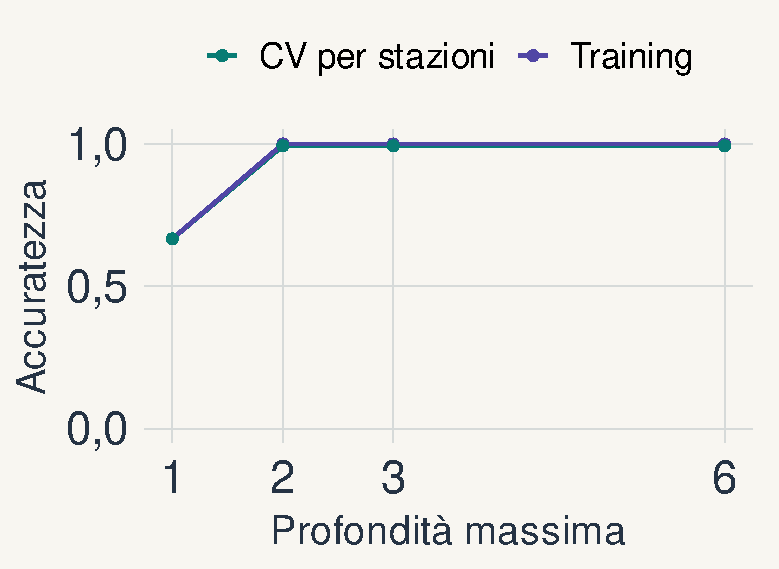
\includegraphics[width=\linewidth,height=6.15cm,keepaspectratio]{Figure/F09.pdf}\par}
\PSmall{Stessi controlli di crescita, profondità diverse. La CV esclude intere stazioni e viene ricalcolata per ogni profondità.}
}};
\node[anchor=north west,inner sep=0] at([xshift=10.85cm,yshift=-2.12cm]current page.north west){\Colonna{8.16cm}{\PBody{Aumentando la profondità da uno a due, l’albero passa da circa due terzi a uno di accuratezza sull’addestramento, mentre la validazione per stazioni raggiunge circa 0,993. Le profondità ulteriori mantengono questi valori nel caso didattico. La figura documenta una separazione molto agevole fra le classi sintetiche e non mostra un peggioramento progressivo della validazione. Il principio generale resta quello di confrontare l’adattamento con prestazioni esterne all’adattamento, evitando di dedurre la generalizzazione dalla sola riuscita sul campione utilizzato.}
}};
\end{tikzpicture}\end{frame}

\begin{frame}[plain]\hypertarget{slide36}{}
\bookmark[level=1,page=36]{Foreste casuali e aggregazione dei voti}
\begin{tikzpicture}[remember picture,overlay]
\PilotChrome{Foreste casuali e aggregazione dei voti}{ALBERI E INSIEMI DI CLASSIFICATORI}{36}{L’aggregazione modifica la regola predittiva e conserva la necessità di verificare il dominio della previsione.}
\node[anchor=north west,inner sep=0] at([xshift=.96cm,yshift=-2.12cm]current page.north west){\Colonna{9.40cm}{{\centering\resizebox{.97\linewidth}{!}{\begin{tikzpicture}[x=1cm,y=-.87cm,every node/.style={font=\fontsize{12.2}{15}\selectfont,text=Ink},arr/.style={-{Stealth[length=2mm]},line width=.8pt,draw=Classical}]\path[use as bounding box] (0,0) rectangle (7.45,6.2);
\draw[draw=Classical,fill=Classical!8,rounded corners=2pt,line width=.7pt] (0.4,0.8) rectangle (2.1,2.2);
\node[anchor=center,text=Ink,font=\fontsize{11}{15}\selectfont,text width=1.5cm,align=center] at (1.25,1.5) {Albero 1};
\draw[arr,draw=Classical] (1.25,2.4)--(3.7,3.7);
\draw[draw=Quantum,fill=Quantum!8,rounded corners=2pt,line width=.7pt] (2.85,0.8) rectangle (4.55,2.2);
\node[anchor=center,text=Ink,font=\fontsize{11}{15}\selectfont,text width=1.5cm,align=center] at (3.7,1.5) {Albero 2};
\draw[arr,draw=Quantum] (3.7,2.4)--(3.7,3.7);
\draw[draw=Measure,fill=Measure!8,rounded corners=2pt,line width=.7pt] (5.3,0.8) rectangle (7.0,2.2);
\node[anchor=center,text=Ink,font=\fontsize{11}{15}\selectfont,text width=1.5cm,align=center] at (6.1499999999999995,1.5) {Albero B};
\draw[arr,draw=Measure] (6.1499999999999995,2.4)--(3.7,3.7);
\draw[draw=Classical,fill=Classical!8,rounded corners=2pt,line width=.7pt] (1,3.9) rectangle (6.4,5.3);
\node[anchor=center,text=Ink,font=\fontsize{12.2}{15}\selectfont,text width=5cm,align=center] at (3.7,4.6) {Voto aggregato};

\end{tikzpicture}}\par}
\PSmall{$h_b(x)$: classe proposta dall’albero b per x; B = 80 alberi. Ogni indicatore vale 1 per un voto alla classe c.}
}};
\node[anchor=north west,inner sep=0] at([xshift=10.85cm,yshift=-2.12cm]current page.north west){\Colonna{8.16cm}{\PBody{Una foresta combina alberi ottenuti introducendo casualità nei campioni e nelle variabili candidate alle suddivisioni. L’aggregazione dei voti può stabilizzare la previsione quando gli errori dei singoli alberi presentano diversità sufficiente. Il laboratorio usa ottanta alberi e due variabili candidate per nodo. Il risultato corretto su tutti i trenta campioni di test riguarda il dataset sintetico e il confronto esplorativo del corso; il numero di alberi non compensa una validazione inadeguata o un cambiamento del dominio di applicazione.}
\par\smallskip{\centering\adjustbox{max width=.98\linewidth}{$\displaystyle \widehat y(x)=\arg\max_c\sum_{b=1}^{B}\mathbf1\{h_b(x)=c\}$}\par\smallskip}
}};
\end{tikzpicture}\end{frame}

\begin{frame}[plain]\hypertarget{slide37}{}
\bookmark[level=1,page=37]{Un albero poco profondo definisce una regola leggibile}
\begin{tikzpicture}[remember picture,overlay]
\PilotChrome{Un albero poco profondo definisce una regola leggibile}{ALBERI E INSIEMI DI CLASSIFICATORI}{37}{Il risultato si riferisce alla distribuzione didattica e alla partizione fissata.}
\node[anchor=north west,inner sep=0] at([xshift=.96cm,yshift=-2.12cm]current page.north west){\Colonna{9.40cm}{\PLabel{Risultati del calcolo in R}
{\fontsize{10.2}{12.8}\selectfont\begin{tabular}{@{}>{\raggedright\arraybackslash}p{0.52\linewidth}@{\hspace{.13cm}}>{\raggedright\arraybackslash}p{0.39\linewidth}@{}}\toprule Grandezza & Valore\\[2.3pt]
\midrule 
Accuratezza & 1\\[2.3pt]
Foglie & 3\\[2.3pt]
\bottomrule\end{tabular}\par}
}};
\node[anchor=north west,inner sep=0] at([xshift=10.85cm,yshift=-2.12cm]current page.north west){\Colonna{8.16cm}{\PBody{Quante foglie bastano a separare le classi di questo campione sintetico?}
\vspace{.4cm}\PInfo{Il risultato si riferisce alla distribuzione didattica e alla partizione fissata. Aumentare la profondità richiede una nuova valutazione interna.}
}};
\node[anchor=north east,inner sep=0] at([xshift=17.1cm,yshift=-12.04cm]current page.north west){\fontsize{7.7}{9}\selectfont \href{https://github.com/marzione00/Lab_Geo/blob/649f7cc577b96bd1044d81e78a2f530813e4f96b/materiali/laboratori/M16/M16_N08.R}{\color{Classical}\bfseries Script R · M16\_N08}};
\end{tikzpicture}\end{frame}

\begin{frame}[plain]\hypertarget{slide38}{}
\bookmark[level=1,page=38]{Alberi e aggregazione di classificatori}
\begin{tikzpicture}[remember picture,overlay]
\PilotChrome{Alberi e aggregazione di classificatori}{ALBERI E INSIEMI DI CLASSIFICATORI}{38}{Confrontare un albero con un insieme di alberi su campioni bootstrap.}
\node[anchor=north west,inner sep=0] at([xshift=.96cm,yshift=-2.12cm]current page.north west){\Colonna{9.40cm}{{\centering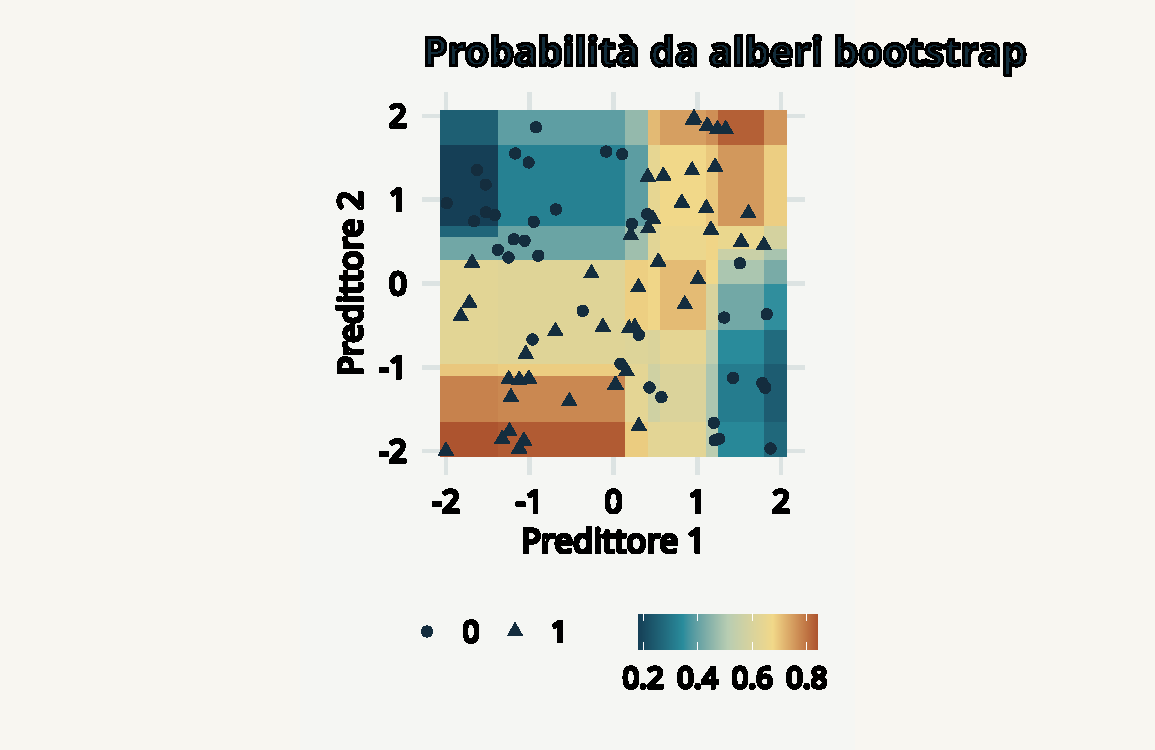
\includegraphics[width=\linewidth,height=6.0cm,keepaspectratio]{Esperimenti/m16-alberi-A.pdf}\par}
\PSmall{Profondità massima: 2. Seme: 17.}
}};
\node[anchor=north west,inner sep=0] at([xshift=10.85cm,yshift=-2.12cm]current page.north west){\Colonna{8.16cm}{\PLabel{Scenario A · simulazione}
\PBody{Un albero di classificazione suddivide lo spazio dei predittori mediante soglie successive, assegnando a ciascuna foglia una probabilità stimata dalla frequenza della classe. Il problema sintetico presenta una relazione non lineare fra due variabili e risposta binaria. Il controllo sulla profondità determina quante divisioni successive possano essere costruite secondo il criterio di impurità di Gini.}
\par\smallskip{\centering\adjustbox{max width=.98\linewidth}{$\displaystyle \widehat p_{bag}(x)=B^{-1}\sum_b\widehat p_b(x)$}\par\smallskip}
\PSmall{B è il numero di alberi, $\hat p_b(x)$ la probabilità stimata dall’albero b e $\hat p_{\mathrm{bag}}(x)$ la loro media. Le probabilità delle foglie sono proporzioni della classe uno nei campioni bootstrap utilizzati per l’adattamento.}
}};
\node[anchor=north east,inner sep=0] at([xshift=17.1cm,yshift=-12.04cm]current page.north west){\fontsize{7.7}{9}\selectfont \href{https://marzione00.github.io/Lab_Geo/\#laboratorio/m16-alberi}{\color{Classical}\bfseries Apri il laboratorio · m16-alberi}};
\end{tikzpicture}\end{frame}

\begin{frame}[plain]\hypertarget{slide39}{}
\bookmark[level=1,page=39]{Confronto | Alberi e aggregazione di classificatori}
\begin{tikzpicture}[remember picture,overlay]
\PilotChrome{Confronto | Alberi e aggregazione di classificatori}{ALBERI E INSIEMI DI CLASSIFICATORI}{39}{L’aggregazione media previsioni di modelli diversi; la profondità governa la complessità delle partizioni.}
\node[anchor=north west,inner sep=0] at([xshift=.96cm,yshift=-2.12cm]current page.north west){\Colonna{9.40cm}{{\centering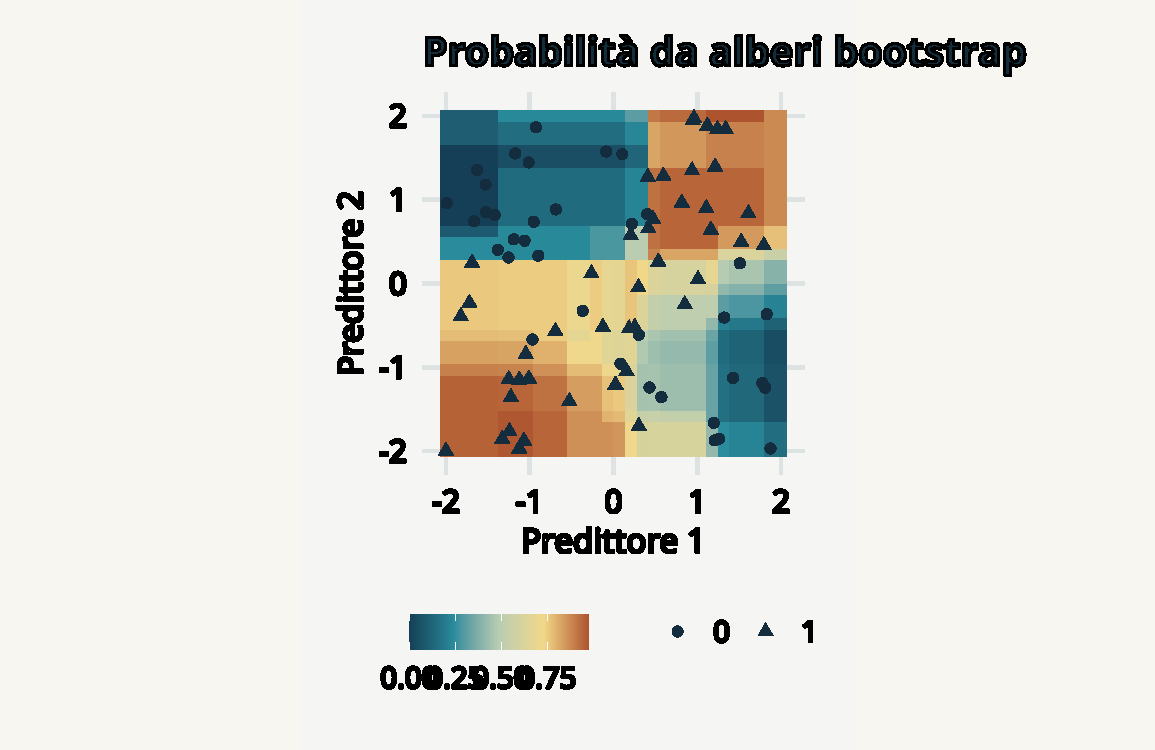
\includegraphics[width=\linewidth,height=5.6cm,keepaspectratio]{Esperimenti/m16-alberi-B.pdf}\par}
\PSmall{Profondità massima: 2 $\to$ 4. Tutti gli altri parametri e il seme sono fissi.}
}};
\node[anchor=north west,inner sep=0] at([xshift=10.85cm,yshift=-2.12cm]current page.north west){\Colonna{8.16cm}{\PLabel{Confronto fra gli scenari}
{\fontsize{10.2}{12.8}\selectfont\begin{tabular}{@{}>{\raggedright\arraybackslash}p{0.48\linewidth}@{\hspace{.13cm}}>{\raggedright\arraybackslash}p{0.224\linewidth}@{\hspace{.13cm}}>{\raggedright\arraybackslash}p{0.224\linewidth}@{}}\toprule Grandezza & A & B\\[2.3pt]
\midrule 
Alberi & 10 & 10\\[2.3pt]
Profondità & 2 & 4\\[2.3pt]
Probabilità media della griglia & 0,556 & 0,544\\[2.3pt]
\bottomrule\end{tabular}\par}
\vspace{.25cm}\PBody{La probabilità media sulla griglia passa da 0,556 a 0,544. Per interpretare questa variazione occorre guardare anche come si ridisegnano le regioni di decisione.}
}};
\node[anchor=north east,inner sep=0] at([xshift=17.1cm,yshift=-12.04cm]current page.north west){\fontsize{7.7}{9}\selectfont \href{https://marzione00.github.io/Lab_Geo/\#laboratorio/m16-alberi}{\color{Classical}\bfseries Apri il laboratorio · m16-alberi}};
\end{tikzpicture}\end{frame}

\begin{frame}[plain]\hypertarget{slide40}{}
\bookmark[level=0,page=40]{Metriche e probabilità}
\bookmark[level=1,page=40]{La stessa accuratezza può nascondere una classe persa}
\begin{tikzpicture}[remember picture,overlay]
\PilotChrome{La stessa accuratezza può nascondere una classe persa}{METRICHE E PROBABILITÀ}{40}{Accompagna l’accuratezza con i conteggi e con una metrica per ciascuna classe.}
\node[anchor=north west,inner sep=0] at([xshift=.96cm,yshift=-2.12cm]current page.north west){\Colonna{9.40cm}{\PLabel{Domanda}
\PBody{Su cento casi ci sono novanta negativi e dieci positivi. Il classificatore assegna sempre la classe negativa. Che prestazioni dichiareresti?}
\vspace{.35cm}\PLabel{Interpretazione}
\PBody{L’accuratezza è 0,9. Il richiamo dei positivi è zero e quello dei negativi è uno. La media dei due richiami è 0,5.}
}};
\node[anchor=north west,inner sep=0] at([xshift=10.85cm,yshift=-2.12cm]current page.north west){\Colonna{8.16cm}{\begin{tcolorbox}[enhanced,arc=1.7mm,boxrule=.6pt,colback=white,colframe=Classical!60!Navy,colbacktitle=Navy,coltitle=white,fonttitle=\bfseries\small,title={R · calcolo riproducibile},left=1.7mm,right=1.3mm,top=1.1mm,bottom=1.1mm,before skip=1mm,after skip=1.0mm]\lstinputlisting[style=GeoR,language=R]{Codice/capitolo-05.R}\end{tcolorbox}
\PLabel{Risultato in R}
\begin{tcolorbox}[colback=GeoTint,colframe=Rule,boxrule=.5pt,arc=1.4mm,left=2mm,right=1mm,top=1mm,bottom=1mm]{\fontsize{9}{12}\selectfont\ttfamily \mbox{accuracy\ bilanciata\ }\\\mbox{\ \ \ \ \ \ \ 0.9\ \ \ \ \ \ \ \ 0.5}}\end{tcolorbox}}};
\end{tikzpicture}\end{frame}

\begin{frame}[plain]\hypertarget{slide41}{}
\bookmark[level=1,page=41]{La matrice di confusione conserva i conteggi}
\begin{tikzpicture}[remember picture,overlay]
\PilotChrome{La matrice di confusione conserva i conteggi}{METRICHE E PROBABILITÀ}{41}{I conteggi e le unità di validazione devono accompagnare qualsiasi percentuale di accuratezza.}
\node[anchor=north west,inner sep=0] at([xshift=.96cm,yshift=-2.12cm]current page.north west){\Colonna{9.40cm}{{\centering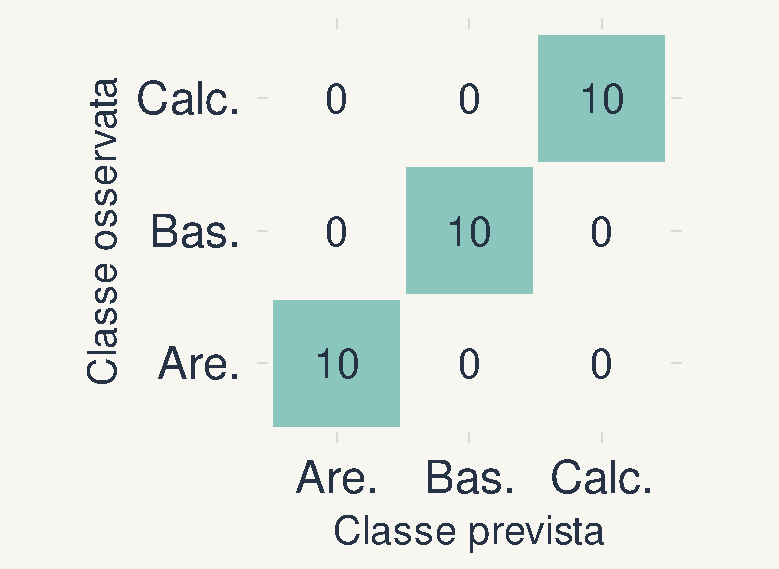
\includegraphics[width=\linewidth,height=6.15cm,keepaspectratio]{Figure/F04.pdf}\par}
\PSmall{a: classe osservata; b: prevista; n = 30. tr(C): somma della diagonale. Are., Bas., Calc.: Arenaria, Basalto, Calcare.}
}};
\node[anchor=north west,inner sep=0] at([xshift=10.85cm,yshift=-2.12cm]current page.north west){\Colonna{8.16cm}{\PBody{Le righe identificano le classi osservate e le colonne quelle previste, mantenendo lo stesso ordine su entrambi gli assi. I valori diagonali contano le classificazioni corrette, mentre le celle esterne mostrano quali classi vengano confuse. Per il centroide a cinque predittori, tutti i trenta campioni sono classificati correttamente, con dieci casi in ciascuna cella diagonale. Il risultato deve essere letto insieme alla facilità del dataset, al numero limitato di stazioni e alla natura esplorativa del riuso del test.}
\par\smallskip{\centering\adjustbox{max width=.98\linewidth}{$\displaystyle C_{ab}=\sum_i\mathbf1\{y_i=a,\widehat y_i=b\},\qquad Acc=\frac{\operatorname{tr}(C)}{n}$}\par\smallskip}
}};
\end{tikzpicture}\end{frame}

\begin{frame}[plain]\hypertarget{slide42}{}
\bookmark[level=1,page=42]{Precisione e richiamo usano denominatori diversi}
\begin{tikzpicture}[remember picture,overlay]
\PilotChrome{Precisione e richiamo usano denominatori diversi}{METRICHE E PROBABILITÀ}{42}{La classe positiva e il denominatore determinano il significato della metrica.}
\node[anchor=north west,inner sep=0] at([xshift=.96cm,yshift=-2.12cm]current page.north west){\Colonna{9.40cm}{{\centering\resizebox{.97\linewidth}{!}{\begin{tikzpicture}[x=1cm,y=-.87cm,every node/.style={font=\fontsize{12.2}{15}\selectfont,text=Ink},arr/.style={-{Stealth[length=2mm]},line width=.8pt,draw=Classical}]\path[use as bounding box] (0,0) rectangle (7.45,6.2);
\draw[draw=Classical,fill=Classical!8,rounded corners=2pt,line width=.7pt] (0.6,0.8) rectangle (6.8,2.5);
\node[anchor=center,text=Ink,font=\fontsize{12.2}{15}\selectfont,text width=6cm,align=center] at (3.7,1.65) {Positivi previsti: $TP+FP$};
\draw[draw=Quantum,fill=Quantum!8,rounded corners=2pt,line width=.7pt] (0.6,3.5) rectangle (6.8,5.2);
\node[anchor=center,text=Ink,font=\fontsize{12.2}{15}\selectfont,text width=6cm,align=center] at (3.7,4.35) {Positivi osservati: $TP+FN$};

\end{tikzpicture}}\par}
\PSmall{TP: veri positivi; FP: falsi positivi; FN: falsi negativi. Classe positiva: Basalto. Nell’esempio TP = 10, FP = FN = 0.}
}};
\node[anchor=north west,inner sep=0] at([xshift=10.85cm,yshift=-2.12cm]current page.north west){\Colonna{8.16cm}{\PBody{Definita Basalto come classe positiva, i veri positivi sono i basalti previsti correttamente; i falsi positivi provengono dalle altre classi, mentre i falsi negativi sono basalti assegnati altrove. La precisione considera l’insieme dei positivi previsti e il richiamo quello dei positivi osservati. Nel caso del centroide entrambi valgono uno, poiché si contano dieci veri positivi e nessun errore. Quando il denominatore è nullo, la metrica risulta indefinita e la convenzione di rappresentazione deve essere dichiarata.}
\par\smallskip{\centering\adjustbox{max width=.98\linewidth}{$\displaystyle \mathrm{Prec}=\frac{TP}{TP+FP},\qquad\mathrm{Rec}=\frac{TP}{TP+FN}$}\par\smallskip}
}};
\end{tikzpicture}\end{frame}

\begin{frame}[plain]\hypertarget{slide43}{}
\bookmark[level=1,page=43]{Sbilanciamento e media dei richiami}
\begin{tikzpicture}[remember picture,overlay]
\PilotChrome{Sbilanciamento e media dei richiami}{METRICHE E PROBABILITÀ}{43}{Una metrica aggregata deve essere accompagnata dalle prestazioni delle classi rilevanti.}
\node[anchor=north west,inner sep=0] at([xshift=.96cm,yshift=-2.12cm]current page.north west){\Colonna{9.40cm}{{\centering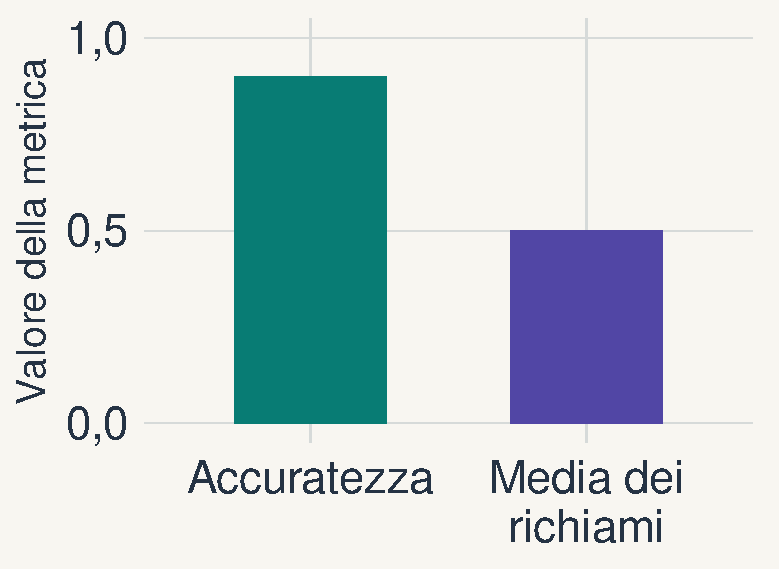
\includegraphics[width=\linewidth,height=6.15cm,keepaspectratio]{Figure/F11.pdf}\par}
\PSmall{K = 2 classi; $TP_c$ e $FN_c$: veri positivi e falsi negativi per c. Novanta A, dieci B; previsione costante A.}
}};
\node[anchor=north west,inner sep=0] at([xshift=10.85cm,yshift=-2.12cm]current page.north west){\Colonna{8.16cm}{\PBody{In un campione artificiale con novanta casi A e dieci casi B, la previsione costante A raggiunge accuratezza pari al novanta per cento, pur lasciando tutti i casi B senza riconoscimento. Il richiamo vale uno per A e zero per B, per cui la loro media è un mezzo. La balanced accuracy assegna uguale peso ai richiami delle classi e rende evidente questo limite. La scelta delle metriche deve comunque riflettere costi, prevalenze e finalità dell’applicazione, conservando i conteggi necessari a interpretarle.}
\par\smallskip{\centering\adjustbox{max width=.98\linewidth}{$\displaystyle BA=\frac1K\sum_{c=1}^{K}\frac{TP_c}{TP_c+FN_c}$}\par\smallskip}
}};
\end{tikzpicture}\end{frame}

\begin{frame}[plain]\hypertarget{slide44}{}
\bookmark[level=1,page=44]{Regressione logistica per una risposta binaria}
\begin{tikzpicture}[remember picture,overlay]
\PilotChrome{Regressione logistica per una risposta binaria}{METRICHE E PROBABILITÀ}{44}{Una probabilità predetta deve essere interpretata rispetto alla specificazione e al dominio del modello.}
\node[anchor=north west,inner sep=0] at([xshift=.96cm,yshift=-2.12cm]current page.north west){\Colonna{9.40cm}{{\centering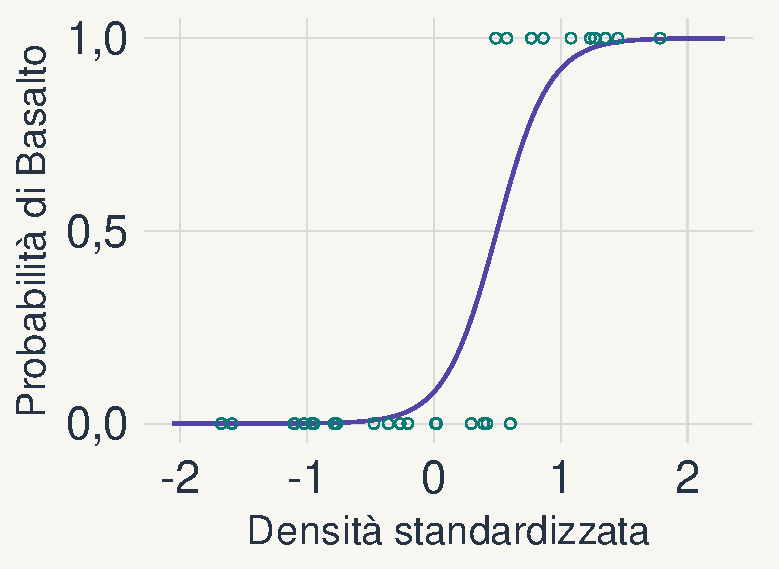
\includegraphics[width=\linewidth,height=6.15cm,keepaspectratio]{Figure/F06.pdf}\par}
\PSmall{z: densità standardizzata; p(z): probabilità di Basalto; $\beta_0,\beta_1$: coefficienti stimati. Cerchi: risposte 0–1 del test.}
}};
\node[anchor=north west,inner sep=0] at([xshift=10.85cm,yshift=-2.12cm]current page.north west){\Colonna{8.16cm}{\PBody{La domanda binaria distingue Basalto dalle altre due classi e usa soltanto la densità standardizzata. Il modello esprime il logaritmo del rapporto fra probabilità positiva e negativa come funzione lineare del predittore, mentre la trasformazione logistica mantiene la probabilità fra zero e uno. La curva viene stimata sui campioni di addestramento e applicata al test. La probabilità rappresenta una previsione condizionata ai dati e al modello, la cui calibrazione richiede una verifica distinta dalla semplice separazione delle classi.}
\par\smallskip{\centering\adjustbox{max width=.98\linewidth}{$\displaystyle \log\frac{p(z)}{1-p(z)}=\beta_0+\beta_1z,\qquad p(z)=\frac1{1+e^{-(\beta_0+\beta_1z)}}$}\par\smallskip}
}};
\end{tikzpicture}\end{frame}

\begin{frame}[plain]\hypertarget{slide45}{}
\bookmark[level=1,page=45]{Soglia e conseguenze della decisione}
\begin{tikzpicture}[remember picture,overlay]
\PilotChrome{Soglia e conseguenze della decisione}{METRICHE E PROBABILITÀ}{45}{La soglia collega probabilità e conseguenze delle decisioni entro ipotesi esplicite.}
\node[anchor=north west,inner sep=0] at([xshift=.96cm,yshift=-2.12cm]current page.north west){\Colonna{9.40cm}{{\centering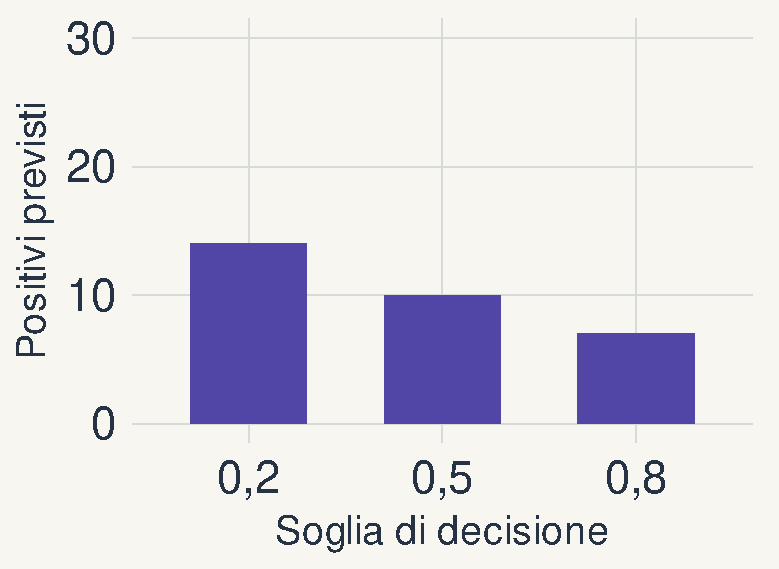
\includegraphics[width=\linewidth,height=6.15cm,keepaspectratio]{Figure/F07.pdf}\par}
\PSmall{$C_{FP}$: costo di un falso positivo; $C_{FN}$: costo di un falso negativo. p: probabilità di Basalto; t: soglia.}
}};
\node[anchor=north west,inner sep=0] at([xshift=10.85cm,yshift=-2.12cm]current page.north west){\Colonna{8.16cm}{\PBody{Trasformare una probabilità in una classe richiede una soglia. Nel test, le soglie 0,2, 0,5 e 0,8 producono rispettivamente quattordici, dieci e sette positivi, perché gli insiemi selezionati si restringono all’aumentare del criterio. In una decisione con costi positivi costanti, probabilità calibrate e costo nullo delle classificazioni corrette, il confronto fra perdita attesa positiva e negativa determina una soglia teorica. La scelta operativa richiede che tali ipotesi e i costi siano pertinenti all’applicazione.}
\par\smallskip{\centering\adjustbox{max width=.98\linewidth}{$\displaystyle \widehat y=\mathbf1\{p\geq t\},\qquad t=\frac{C_{FP}}{C_{FP}+C_{FN}}$}\par\smallskip}
}};
\end{tikzpicture}\end{frame}

\begin{frame}[plain]\hypertarget{slide46}{}
\bookmark[level=1,page=46]{Il punteggio di Brier valuta le probabilità}
\begin{tikzpicture}[remember picture,overlay]
\PilotChrome{Il punteggio di Brier valuta le probabilità}{METRICHE E PROBABILITÀ}{46}{Un punteggio probabilistico richiede riferimenti e condizioni di confronto dichiarati.}
\node[anchor=north west,inner sep=0] at([xshift=.96cm,yshift=-2.12cm]current page.north west){\Colonna{9.40cm}{\PLabel{Metodo}
\PBody{Il punteggio di Brier è la media degli scarti quadratici fra probabilità prevista e risposta binaria. Penalizza previsioni confidenti che risultano errate e utilizza l’intera scala probabilistica, mentre l’accuratezza dipende da una soglia. Per la logistica del laboratorio vale circa 0,04286 sui trenta campioni di test. Il valore va confrontato con riferimenti pertinenti alla stessa popolazione e prevalenza; da solo non descrive quali classi o intervalli di probabilità contribuiscano maggiormente all’errore.}
}};
\node[anchor=north west,inner sep=0] at([xshift=10.85cm,yshift=-2.12cm]current page.north west){\Colonna{8.16cm}{\PLabel{Formalismo}
\par\smallskip{\centering\adjustbox{max width=.98\linewidth}{$\displaystyle BS=\frac1n\sum_{i=1}^{n}(p_i-y_i)^2,\qquad 0\leq BS\leq1$}\par\smallskip}
\PLabel{Interpretazione}
\PBody{$p_i$: probabilità prevista di Basalto; $y_i=1$ per Basalto, 0 altrimenti; n = 30. Una previsione perfetta ottiene punteggio nullo. Un riferimento costante può usare la prevalenza stimata sull’addestramento. La prevalenza osservata nel test descrive invece quel campione e non deve essere utilizzata per adattare il riferimento da valutare.}
}};
\end{tikzpicture}\end{frame}

\begin{frame}[plain]\hypertarget{slide47}{}
\bookmark[level=1,page=47]{Dal modello alle probabilità verificabili}
\begin{tikzpicture}[remember picture,overlay]
\PilotChrome{Dal modello alle probabilità verificabili}{METRICHE E PROBABILITÀ}{47}{Il controllo numerico rende verificabile il calcolo senza attribuire precisione aggiuntiva alla valutazione predittiva.}
\node[anchor=north west,inner sep=0] at([xshift=.96cm,yshift=-2.12cm]current page.north west){\Colonna{9.40cm}{\begin{tcolorbox}[enhanced,arc=1.7mm,boxrule=.6pt,colback=white,colframe=Classical!60!Navy,colbacktitle=Navy,coltitle=white,fonttitle=\bfseries\small,title={R · procedura},left=1.7mm,right=1.3mm,top=1.1mm,bottom=1.1mm,before skip=1mm,after skip=1.0mm]\lstinputlisting[style=GeoR,language=R]{Codice/lettura-25.R}\end{tcolorbox}
}};
\node[anchor=north west,inner sep=0] at([xshift=10.85cm,yshift=-2.12cm]current page.north west){\Colonna{8.16cm}{\PBody{Il frammento ricostruisce la trasformazione della densità, adatta la risposta binaria sull’addestramento e calcola il punteggio sui campioni esclusi. La tolleranza verifica la concordanza con il valore atteso dell’esercizio, mantenendo distinto il controllo numerico dall’incertezza della prestazione. Per una nuova applicazione si conserverebbero coefficienti, media e deviazione standard del predittore, insieme alla definizione della classe positiva e alle condizioni nelle quali le misure sono disponibili.}
}};
\end{tikzpicture}\end{frame}

\begin{frame}[plain]\hypertarget{slide48}{}
\bookmark[level=1,page=48]{Calibrazione e numerosità degli intervalli}
\begin{tikzpicture}[remember picture,overlay]
\PilotChrome{Calibrazione e numerosità degli intervalli}{METRICHE E PROBABILITÀ}{48}{La lettura della calibrazione dipende dalla numerosità e dalla struttura delle osservazioni in ogni intervallo.}
\node[anchor=north west,inner sep=0] at([xshift=.96cm,yshift=-2.12cm]current page.north west){\Colonna{9.40cm}{{\centering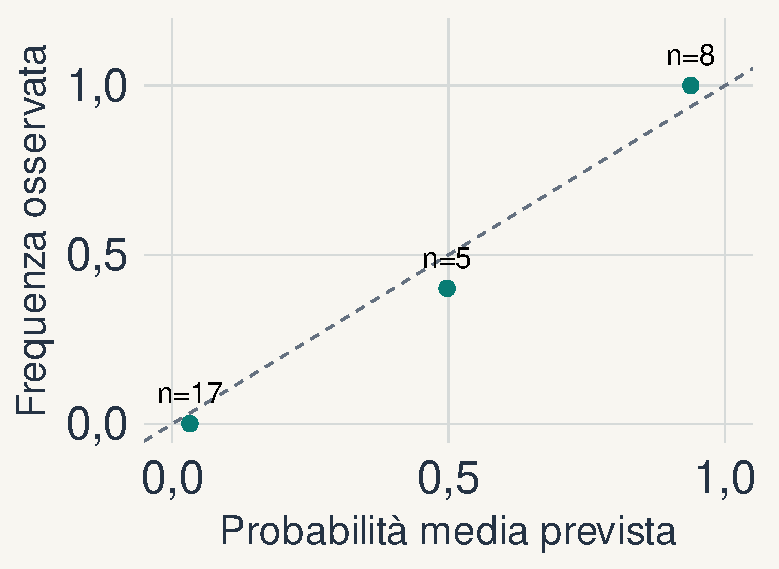
\includegraphics[width=\linewidth,height=6.15cm,keepaspectratio]{Figure/F08.pdf}\par}
\PSmall{Intervalli delimitati da 1/3 e 2/3. Le etichette riportano il numero di casi che sostiene ciascun punto.}
}};
\node[anchor=north west,inner sep=0] at([xshift=10.85cm,yshift=-2.12cm]current page.north west){\Colonna{8.16cm}{\PBody{Le probabilità vengono suddivise in tre intervalli, entro i quali si confrontano probabilità media e frequenza osservata di Basalto. I gruppi contengono rispettivamente diciassette, cinque e otto campioni, per cui soprattutto il punto centrale può variare molto al cambiare di poche osservazioni. La diagonale rappresenta la corrispondenza ideale nel riassunto per intervalli. Questa rappresentazione descrittiva usa soltanto tre stazioni di test e richiede dati ulteriori per valutare stabilmente la calibrazione in un contesto di applicazione.}
}};
\end{tikzpicture}\end{frame}

\begin{frame}[plain]\hypertarget{slide49}{}
\bookmark[level=1,page=49]{Un forte sbilanciamento altera il giudizio globale}
\begin{tikzpicture}[remember picture,overlay]
\PilotChrome{Un forte sbilanciamento altera il giudizio globale}{METRICHE E PROBABILITÀ}{49}{La differenza fra 0,9 e 0,5 fa emergere il fallimento sulla classe rara.}
\node[anchor=north west,inner sep=0] at([xshift=.96cm,yshift=-2.12cm]current page.north west){\Colonna{9.40cm}{\PLabel{Risultati del calcolo in R}
{\fontsize{10.2}{12.8}\selectfont\begin{tabular}{@{}>{\raggedright\arraybackslash}p{0.52\linewidth}@{\hspace{.13cm}}>{\raggedright\arraybackslash}p{0.39\linewidth}@{}}\toprule Grandezza & Valore\\[2.3pt]
\midrule 
Accuratezza & 0,9\\[2.3pt]
Acc. bilanciata & 0,5\\[2.3pt]
\bottomrule\end{tabular}\par}
}};
\node[anchor=north west,inner sep=0] at([xshift=10.85cm,yshift=-2.12cm]current page.north west){\Colonna{8.16cm}{\PBody{Come cambia il giudizio passando dalla quota di classificazioni corrette alla media dei richiami?}
\vspace{.4cm}\PInfo{La differenza fra 0,9 e 0,5 fa emergere il fallimento sulla classe rara. La misura pertinente dipende dal costo dell’errore e dalla domanda applicativa.}
}};
\node[anchor=north east,inner sep=0] at([xshift=17.1cm,yshift=-12.04cm]current page.north west){\fontsize{7.7}{9}\selectfont \href{https://github.com/marzione00/Lab_Geo/blob/649f7cc577b96bd1044d81e78a2f530813e4f96b/materiali/laboratori/M16/M16_N14.R}{\color{Classical}\bfseries Script R · M16\_N14}};
\end{tikzpicture}\end{frame}

\begin{frame}[plain]\hypertarget{slide50}{}
\bookmark[level=1,page=50]{La soglia decide quanti casi vengono segnalati}
\begin{tikzpicture}[remember picture,overlay]
\PilotChrome{La soglia decide quanti casi vengono segnalati}{METRICHE E PROBABILITÀ}{50}{Il numero di positivi scende al crescere della soglia.}
\node[anchor=north west,inner sep=0] at([xshift=.96cm,yshift=-2.12cm]current page.north west){\Colonna{9.40cm}{\PLabel{Risultati del calcolo in R}
{\fontsize{10.2}{12.8}\selectfont\begin{tabular}{@{}>{\raggedright\arraybackslash}p{0.44\linewidth}@{\hspace{.13cm}}>{\raggedright\arraybackslash}p{0.48\linewidth}@{}}\toprule Soglia & n positivi\\[2.3pt]
\midrule 
0,2 & 14\\[2.3pt]
0,5 & 10\\[2.3pt]
0,8 & 7\\[2.3pt]
\bottomrule\end{tabular}\par}
}};
\node[anchor=north west,inner sep=0] at([xshift=10.85cm,yshift=-2.12cm]current page.north west){\Colonna{8.16cm}{\PBody{Quante segnalazioni si ottengono usando soglie via via più alte sulle stesse probabilità?}
\vspace{.4cm}\PInfo{Il numero di positivi scende al crescere della soglia. Il conteggio, da solo, non distingue i veri positivi dai falsi positivi.}
}};
\node[anchor=north east,inner sep=0] at([xshift=17.1cm,yshift=-12.04cm]current page.north west){\fontsize{7.7}{9}\selectfont \href{https://github.com/marzione00/Lab_Geo/blob/649f7cc577b96bd1044d81e78a2f530813e4f96b/materiali/laboratori/M16/M16_N16.R}{\color{Classical}\bfseries Script R · M16\_N16}};
\end{tikzpicture}\end{frame}

\begin{frame}[plain]\hypertarget{slide51}{}
\bookmark[level=1,page=51]{La calibrazione confronta probabilità e frequenze}
\begin{tikzpicture}[remember picture,overlay]
\PilotChrome{La calibrazione confronta probabilità e frequenze}{METRICHE E PROBABILITÀ}{51}{La probabilità media si confronta con la quota di basalti nello stesso gruppo.}
\node[anchor=north west,inner sep=0] at([xshift=.96cm,yshift=-2.12cm]current page.north west){\Colonna{9.40cm}{\PLabel{Risultati del calcolo in R}
{\fontsize{10.2}{12.8}\selectfont\begin{tabular}{@{}>{\raggedright\arraybackslash}p{0.31\linewidth}@{\hspace{.13cm}}>{\raggedright\arraybackslash}p{0.29\linewidth}@{\hspace{.13cm}}>{\raggedright\arraybackslash}p{0.32\linewidth}@{}}\toprule Gruppo & Probabilità & Frazione osservata\\[2.3pt]
\midrule 
(-Inf,0.333] & 0,031642 & 0\\[2.3pt]
(0.333,0.667] & 0,49742 & 0,4\\[2.3pt]
(0.667, Inf] & 0,93889 & 1\\[2.3pt]
\bottomrule\end{tabular}\par}
}};
\node[anchor=north west,inner sep=0] at([xshift=10.85cm,yshift=-2.12cm]current page.north west){\Colonna{8.16cm}{\PBody{Cosa si osserva raggruppando le probabilità previste per ampiezza?}
\vspace{.4cm}\PInfo{La probabilità media si confronta con la quota di basalti nello stesso gruppo. Nei gruppi piccoli una singola osservazione può spostare molto quella quota.}
}};
\node[anchor=north east,inner sep=0] at([xshift=17.1cm,yshift=-12.04cm]current page.north west){\fontsize{7.7}{9}\selectfont \href{https://github.com/marzione00/Lab_Geo/blob/649f7cc577b96bd1044d81e78a2f530813e4f96b/materiali/laboratori/M16/M16_N17.R}{\color{Classical}\bfseries Script R · M16\_N17}};
\end{tikzpicture}\end{frame}

\begin{frame}[plain]\hypertarget{slide52}{}
\bookmark[level=1,page=52]{Soglia, discriminazione e calibrazione}
\begin{tikzpicture}[remember picture,overlay]
\PilotChrome{Soglia, discriminazione e calibrazione}{METRICHE E PROBABILITÀ}{52}{Separare probabilità previste e decisione binaria.}
\node[anchor=north west,inner sep=0] at([xshift=.96cm,yshift=-2.12cm]current page.north west){\Colonna{9.40cm}{{\centering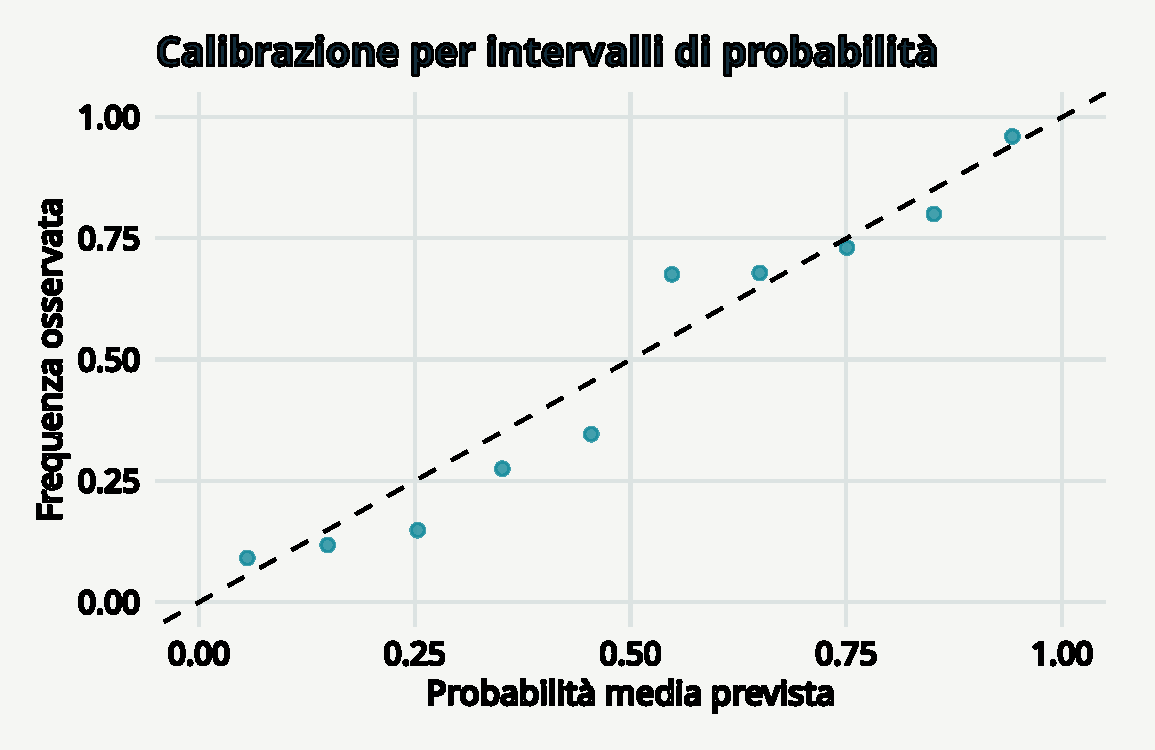
\includegraphics[width=\linewidth,height=6.0cm,keepaspectratio]{Esperimenti/m16-metriche-A.pdf}\par}
\PSmall{Soglia decisionale: 0,5. Seme: 17.}
}};
\node[anchor=north west,inner sep=0] at([xshift=10.85cm,yshift=-2.12cm]current page.north west){\Colonna{8.16cm}{\PLabel{Scenario A · simulazione}
\PBody{Una previsione probabilistica e una decisione binaria rispondono a valutazioni differenti. L’esperimento genera risposte da probabilità logistiche note e modifica le probabilità dichiarate moltiplicandone il logit. Un controllo separato stabilisce la soglia con cui trasformare tali probabilità in classi, rendendo confrontabili calibrazione e conseguenze della decisione.}
\par\smallskip{\centering\adjustbox{max width=.98\linewidth}{$\displaystyle \operatorname{Brier}=n^{-1}\sum_i(p_i-y_i)^2$}\par\smallskip}
\PSmall{$p_i$ è la probabilità dichiarata per l’osservazione i, $y_i$ la risposta binaria e n la numerosità. Il Brier score è la media dei quadrati degli scarti fra probabilità e risposte; valori inferiori indicano previsioni probabilistiche migliori nel campione valutato.}
}};
\node[anchor=north east,inner sep=0] at([xshift=17.1cm,yshift=-12.04cm]current page.north west){\fontsize{7.7}{9}\selectfont \href{https://marzione00.github.io/Lab_Geo/\#laboratorio/m16-metriche}{\color{Classical}\bfseries Apri il laboratorio · m16-metriche}};
\end{tikzpicture}\end{frame}

\begin{frame}[plain]\hypertarget{slide53}{}
\bookmark[level=1,page=53]{Confronto | Soglia, discriminazione e calibrazione}
\begin{tikzpicture}[remember picture,overlay]
\PilotChrome{Confronto | Soglia, discriminazione e calibrazione}{METRICHE E PROBABILITÀ}{53}{Una soglia modifica le decisioni, mentre la calibrazione riguarda il significato delle probabilità.}
\node[anchor=north west,inner sep=0] at([xshift=.96cm,yshift=-2.12cm]current page.north west){\Colonna{9.40cm}{{\centering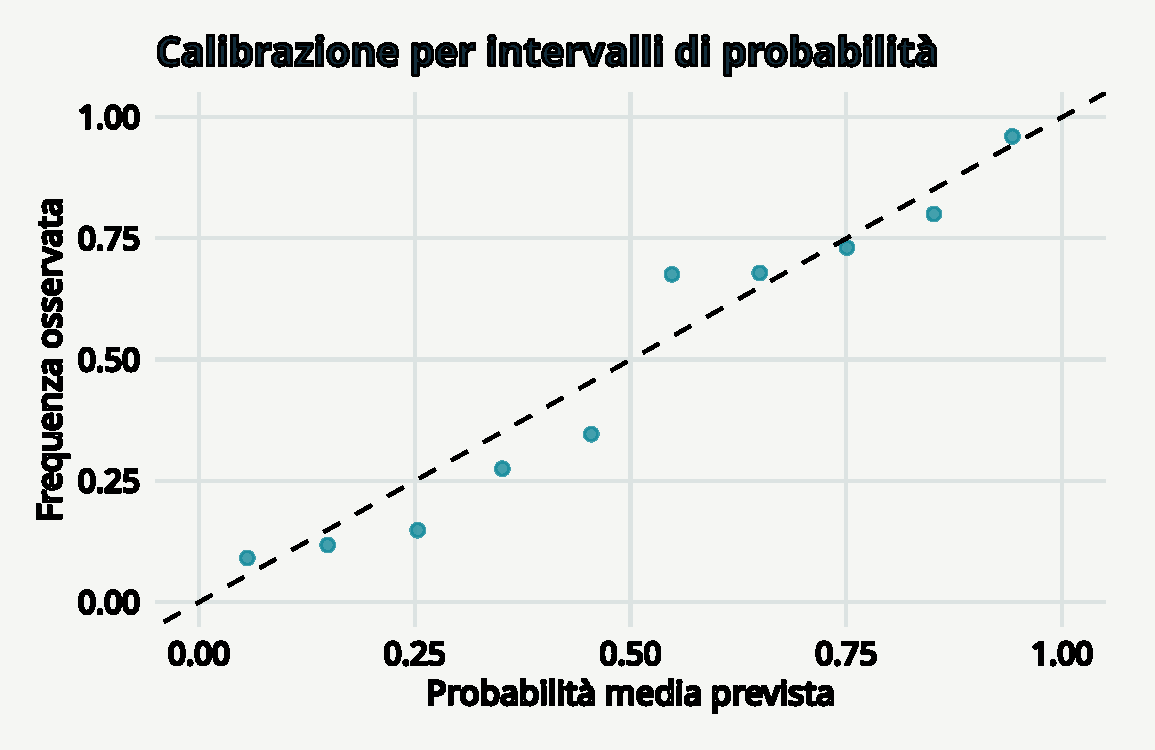
\includegraphics[width=\linewidth,height=5.6cm,keepaspectratio]{Esperimenti/m16-metriche-B.pdf}\par}
\PSmall{Soglia decisionale: 0,5 $\to$ 0,75. Tutti gli altri parametri e il seme sono fissi.}
}};
\node[anchor=north west,inner sep=0] at([xshift=10.85cm,yshift=-2.12cm]current page.north west){\Colonna{8.16cm}{\PLabel{Confronto fra gli scenari}
{\fontsize{10.2}{12.8}\selectfont\begin{tabular}{@{}>{\raggedright\arraybackslash}p{0.48\linewidth}@{\hspace{.13cm}}>{\raggedright\arraybackslash}p{0.224\linewidth}@{\hspace{.13cm}}>{\raggedright\arraybackslash}p{0.224\linewidth}@{}}\toprule Grandezza & A & B\\[2.3pt]
\midrule 
Veri positivi & 115 & 61\\[2.3pt]
Falsi positivi & 36 & 10\\[2.3pt]
Veri negativi & 119 & 145\\[2.3pt]
Falsi negativi & 30 & 84\\[2.3pt]
Sensibilità & 0,793 & 0,421\\[2.3pt]
Specificità & 0,768 & 0,935\\[2.3pt]
Brier score & 0,168 & 0,168\\[2.3pt]
\bottomrule\end{tabular}\par}
\vspace{.25cm}\PBody{Alzando la soglia da 0,50 a 0,75 diminuiscono sia i veri sia i falsi positivi. Il Brier score è invariato perché usa le probabilità prima della soglia.}
}};
\node[anchor=north east,inner sep=0] at([xshift=17.1cm,yshift=-12.04cm]current page.north west){\fontsize{7.7}{9}\selectfont \href{https://marzione00.github.io/Lab_Geo/\#laboratorio/m16-metriche}{\color{Classical}\bfseries Apri il laboratorio · m16-metriche}};
\end{tikzpicture}\end{frame}

\begin{frame}[plain]\hypertarget{slide54}{}
\bookmark[level=0,page=54]{Diagnostica e trasferibilità}
\bookmark[level=1,page=54]{Una probabilità richiede una verifica nel nuovo territorio}
\begin{tikzpicture}[remember picture,overlay]
\PilotChrome{{\fontsize{17.3}{19}\selectfont Una probabilità richiede una verifica nel nuovo territorio}}{DIAGNOSTICA E TRASFERIBILITÀ}{54}{La calibrazione riguarda una popolazione e una modalità di acquisizione dichiarate.}
\node[anchor=north west,inner sep=0] at([xshift=.96cm,yshift=-2.12cm]current page.north west){\Colonna{9.40cm}{\PLabel{Domanda}
\PBody{Quattro stazioni ricevono probabilità 0,8, 0,7, 0,2 e 0,1. Lo stesso modello viene trasferito a un contesto in cui cambiano gli esiti osservati.}
\vspace{.35cm}\PLabel{Interpretazione}
\PBody{Il punteggio di Brier è la media degli scarti quadratici. Aumenta quando le probabilità trasferite si allontanano dai nuovi esiti.}
}};
\node[anchor=north west,inner sep=0] at([xshift=10.85cm,yshift=-2.12cm]current page.north west){\Colonna{8.16cm}{\begin{tcolorbox}[enhanced,arc=1.7mm,boxrule=.6pt,colback=white,colframe=Classical!60!Navy,colbacktitle=Navy,coltitle=white,fonttitle=\bfseries\small,title={R · calcolo riproducibile},left=1.7mm,right=1.3mm,top=1.1mm,bottom=1.1mm,before skip=1mm,after skip=1.0mm]\lstinputlisting[style=GeoR,language=R]{Codice/capitolo-06.R}\end{tcolorbox}
\PLabel{Risultato in R}
\begin{tcolorbox}[colback=GeoTint,colframe=Rule,boxrule=.5pt,arc=1.4mm,left=2mm,right=1mm,top=1mm,bottom=1mm]{\fontsize{9}{12}\selectfont\ttfamily \mbox{orig\ nuovo\ }\\\mbox{0.045\ 0.345}}\end{tcolorbox}}};
\end{tikzpicture}\end{frame}

\begin{frame}[plain]\hypertarget{slide55}{}
\bookmark[level=1,page=55]{Permutare un predittore per esaminare il modello}
\begin{tikzpicture}[remember picture,overlay]
\PilotChrome{Permutare un predittore per esaminare il modello}{DIAGNOSTICA E TRASFERIBILITÀ}{55}{L’importanza predittiva dipende da modello, dati e perturbazione applicata; la sua interpretazione causale richiede altro.}
\node[anchor=north west,inner sep=0] at([xshift=.96cm,yshift=-2.12cm]current page.north west){\Colonna{9.40cm}{{\centering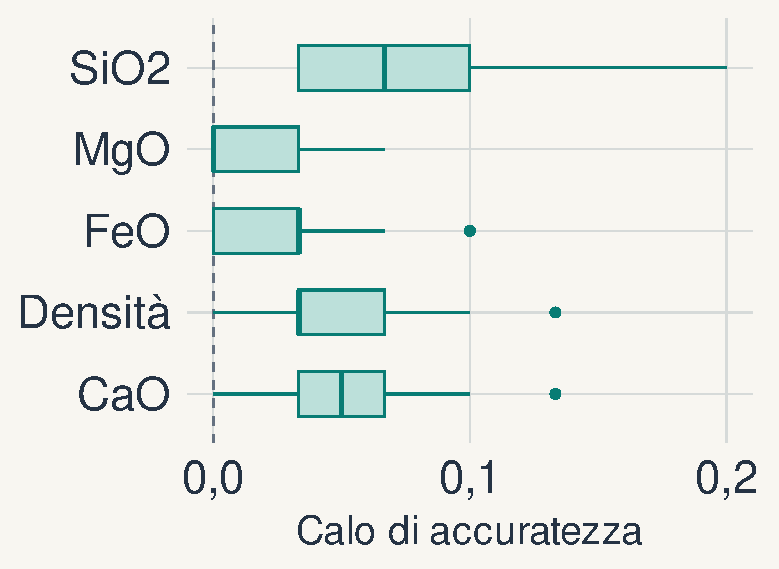
\includegraphics[width=\linewidth,height=6.15cm,keepaspectratio]{Figure/F10.pdf}\par}
\PSmall{$Acc_{base}$: accuratezza originaria; $Acc_{perm(j)}$: dopo la permutazione della variabile j. Trenta repliche per variabile, modello fisso.}
}};
\node[anchor=north west,inner sep=0] at([xshift=10.85cm,yshift=-2.12cm]current page.north west){\Colonna{8.16cm}{\PBody{L’importanza per permutazione confronta la prestazione originaria con quella ottenuta rimescolando un predittore, mantenendo fisso il classificatore. Il confronto ripete trenta permutazioni per variabile, mostrando la variabilità del calo di accuratezza. La procedura rompe associazioni fra predittori e può generare combinazioni lontane dal dominio dei dati, specialmente in presenza di correlazioni. Il risultato riguarda la sensibilità di questo modello e di questo campione; il laboratorio lo utilizza come diagnosi illustrativa, senza tornare a selezionare variabili sul test.}
\par\smallskip{\centering\adjustbox{max width=.98\linewidth}{$\displaystyle I_j=Acc_{base}-Acc_{perm(j)}$}\par\smallskip}
}};
\end{tikzpicture}\end{frame}

\begin{frame}[plain]\hypertarget{slide56}{}
\bookmark[level=1,page=56]{Informazione della risposta nascosta nei predittori}
\begin{tikzpicture}[remember picture,overlay]
\PilotChrome{Informazione della risposta nascosta nei predittori}{DIAGNOSTICA E TRASFERIBILITÀ}{56}{Ogni predittore deve essere disponibile nel momento e nelle condizioni in cui la previsione verrà richiesta.}
\node[anchor=north west,inner sep=0] at([xshift=.96cm,yshift=-2.12cm]current page.north west){\Colonna{9.40cm}{{\centering\resizebox{.97\linewidth}{!}{\begin{tikzpicture}[x=1cm,y=-.87cm,every node/.style={font=\fontsize{12.2}{15}\selectfont,text=Ink},arr/.style={-{Stealth[length=2mm]},line width=.8pt,draw=Classical}]\path[use as bounding box] (0,0) rectangle (7.45,6.2);
\draw[draw=Classical,fill=Classical!8,rounded corners=2pt,line width=.7pt] (0.6,0.6) rectangle (6.8,1.8);
\node[anchor=center,text=Ink,font=\fontsize{12.2}{15}\selectfont,text width=6cm,align=center] at (3.7,1.2) {Classe osservata $Y$};
\draw[arr,draw=Measure] (3.7,2)--(3.7,2.7);
\draw[draw=Measure,fill=Measure!8,rounded corners=2pt,line width=.7pt] (0.6,2.9) rectangle (6.8,4.1);
\node[anchor=center,text=Ink,font=\fontsize{12.2}{15}\selectfont,text width=6cm,align=center] at (3.7,3.5) {Predittore costruito da $Y$};
\draw[arr,draw=Measure] (3.7,4.3)--(3.7,4.9);
\node[anchor=center,text=Ink,font=\fontsize{11.5}{15}\selectfont,text width=6.7cm,align=center] at (3.7,5.5) {Accuratezza perfetta per costruzione};

\end{tikzpicture}}\par}
}};
\node[anchor=north west,inner sep=0] at([xshift=10.85cm,yshift=-2.12cm]current page.north west){\Colonna{8.16cm}{\PBody{Una variabile che codifica direttamente la classe consente una previsione perfetta perché trasferisce la risposta nel problema predittivo. Il controesempio rende evidente una contaminazione che, nelle applicazioni, può essere meno riconoscibile: identificativi costruiti dalle etichette, misure disponibili soltanto dopo la diagnosi o sintesi calcolate utilizzando anche i dati esclusi. Il controllo della disponibilità temporale e della provenienza di ogni predittore precede l’adattamento, poiché una buona metrica può convivere con una domanda predittiva formulata in modo circolare.}
}};
\end{tikzpicture}\end{frame}

\begin{frame}[plain]\hypertarget{slide57}{}
\bookmark[level=1,page=57]{Scheda del modello e limiti dell’esperimento}
\begin{tikzpicture}[remember picture,overlay]
\PilotChrome{Scheda del modello e limiti dell’esperimento}{DIAGNOSTICA E TRASFERIBILITÀ}{57}{La scheda del modello deve rendere ricostruibili sia la previsione sia l’evidenza che ne sostiene l’impiego.}
\node[anchor=north west,inner sep=0] at([xshift=.96cm,yshift=-2.12cm]current page.north west){\Colonna{9.40cm}{\PLabel{Metodo}
\PBody{La scheda finale riporta classi, predittori, unità, trasformazioni, algoritmo, regole di selezione, unità di validazione e conteggi delle prestazioni. Il centroide del laboratorio utilizza cinque variabili standardizzate e viene valutato su tre stazioni sintetiche, con accuratezza uno sui trenta provini. La forte separazione delle classi limita il confronto fra metodi, mentre il riuso didattico del test impedisce di presentare l’intero percorso come una selezione seguita da un’unica verifica indipendente. Il trasferimento a dati reali richiede campioni e protocolli ulteriori.}
}};
\node[anchor=north west,inner sep=0] at([xshift=10.85cm,yshift=-2.12cm]current page.north west){\Colonna{8.16cm}{\PLabel{Interpretazione}
\PBody{I laboratori N01–N05 costruiscono dati, separazione e centroide; N06–N12 confrontano vicini, logistica, alberi e validazione; N13–N17 sviluppano metriche e probabilità; N18–N20 completano diagnostica, contaminazione e scheda. L’esercizio conclusivo definisca un nuovo protocollo prima di generare ulteriori stazioni di prova.}
}};
\end{tikzpicture}\end{frame}

\begin{frame}[plain]\hypertarget{slide58}{}
\bookmark[level=1,page=58]{Una permutazione misura la dipendenza del modello}
\begin{tikzpicture}[remember picture,overlay]
\PilotChrome{Una permutazione misura la dipendenza del modello}{DIAGNOSTICA E TRASFERIBILITÀ}{58}{Il confronto dipende dal classificatore e dai dati valutati.}
\node[anchor=north west,inner sep=0] at([xshift=.96cm,yshift=-2.12cm]current page.north west){\Colonna{9.40cm}{\PLabel{Risultati del calcolo in R}
{\fontsize{10.2}{12.8}\selectfont\begin{tabular}{@{}>{\raggedright\arraybackslash}p{0.44\linewidth}@{\hspace{.13cm}}>{\raggedright\arraybackslash}p{0.48\linewidth}@{}}\toprule variabile & calo accuracy\\[2.3pt]
\midrule 
SiO2 & 0,066667\\[2.3pt]
CaO & 0,033333\\[2.3pt]
MgO & 0\\[2.3pt]
FeO & 0,066667\\[2.3pt]
densita & 0,066667\\[2.3pt]
\bottomrule\end{tabular}\par}
}};
\node[anchor=north west,inner sep=0] at([xshift=10.85cm,yshift=-2.12cm]current page.north west){\Colonna{8.16cm}{\PBody{Quanto cala l’accuratezza permutando un predittore alla volta?}
\vspace{.4cm}\PInfo{Il confronto dipende dal classificatore e dai dati valutati. Predittori correlati possono sostituirsi e ridurre il calo osservato per una singola variabile.}
}};
\node[anchor=north east,inner sep=0] at([xshift=17.1cm,yshift=-12.04cm]current page.north west){\fontsize{7.7}{9}\selectfont \href{https://github.com/marzione00/Lab_Geo/blob/649f7cc577b96bd1044d81e78a2f530813e4f96b/materiali/laboratori/M16/M16_N18.R}{\color{Classical}\bfseries Script R · M16\_N18}};
\end{tikzpicture}\end{frame}

\begin{frame}[plain]\hypertarget{slide59}{}
\bookmark[level=1,page=59]{Trasferibilità e cambiamento della relazione}
\begin{tikzpicture}[remember picture,overlay]
\PilotChrome{Trasferibilità e cambiamento della relazione}{DIAGNOSTICA E TRASFERIBILITÀ}{59}{Valutare un modello su una popolazione differente.}
\node[anchor=north west,inner sep=0] at([xshift=.96cm,yshift=-2.12cm]current page.north west){\Colonna{9.40cm}{{\centering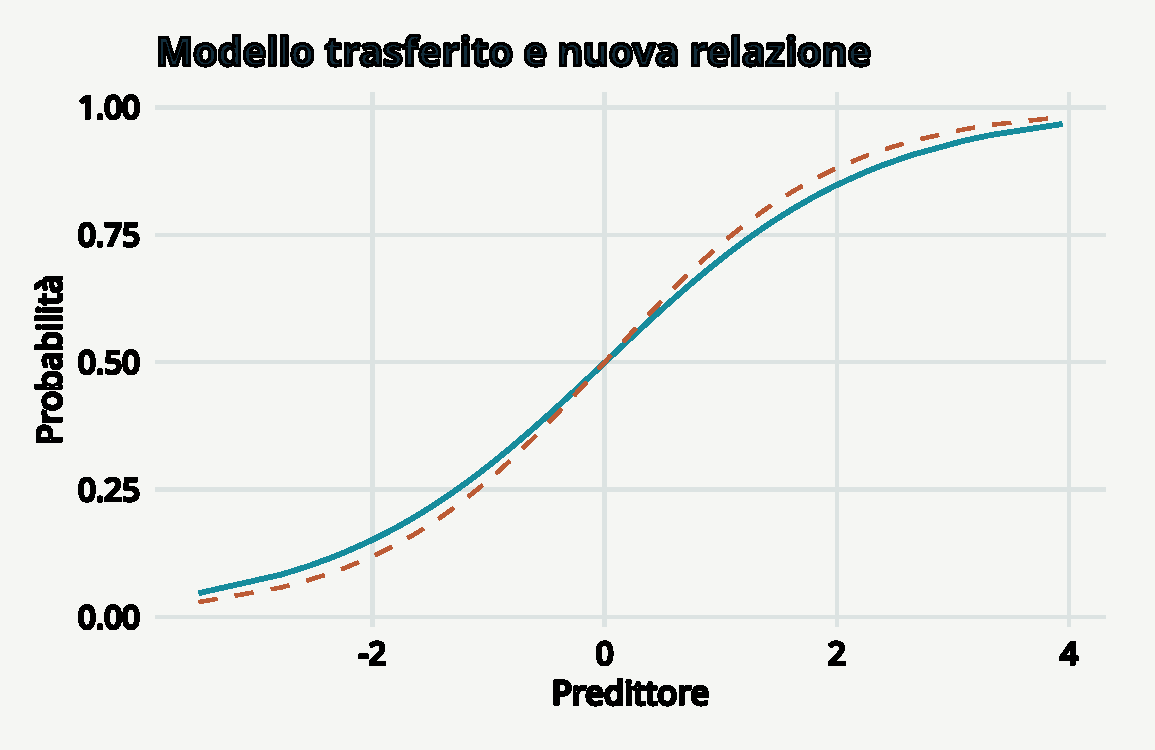
\includegraphics[width=\linewidth,height=6.0cm,keepaspectratio]{Esperimenti/m16-trasferimento-A.pdf}\par}
\PSmall{Pendenza nel nuovo territorio: 1. Seme: 17.}
}};
\node[anchor=north west,inner sep=0] at([xshift=10.85cm,yshift=-2.12cm]current page.north west){\Colonna{8.16cm}{\PLabel{Scenario A · simulazione}
\PBody{Un modello può perdere accuratezza quando la relazione fra predittori e risposta cambia nel territorio di destinazione. L’esperimento adatta una regressione logistica a un primo campione e la applica a una nuova popolazione, della quale il controllo modifica la pendenza della relazione probabilistica. La distribuzione del predittore resta invariata, isolando il cambiamento della risposta condizionata.}
\par\smallskip{\centering\adjustbox{max width=.98\linewidth}{$\displaystyle P_{train}(Y\mid X)\quad\hbox{e}\quad P_{nuovo}(Y\mid X)$}\par\smallskip}
\PSmall{$P_{\mathrm{train}}(Y\mid X)$ è la distribuzione della risposta condizionata ai predittori nel dominio di addestramento; $P_{\mathrm{nuovo}}(Y\mid X)$ è quella del dominio di destinazione. Il controllo modifica la seconda mantenendo fisso il classificatore già stimato.}
}};
\node[anchor=north east,inner sep=0] at([xshift=17.1cm,yshift=-12.04cm]current page.north west){\fontsize{7.7}{9}\selectfont \href{https://marzione00.github.io/Lab_Geo/\#laboratorio/m16-trasferimento}{\color{Classical}\bfseries Apri il laboratorio · m16-trasferimento}};
\end{tikzpicture}\end{frame}

\begin{frame}[plain]\hypertarget{slide60}{}
\bookmark[level=1,page=60]{Confronto | Trasferibilità e cambiamento della relazione}
\begin{tikzpicture}[remember picture,overlay]
\PilotChrome{Confronto | Trasferibilità e cambiamento della relazione}{DIAGNOSTICA E TRASFERIBILITÀ}{60}{La validazione interna riguarda il dominio osservato; il trasferimento richiede una verifica coerente con il nuovo contesto.}
\node[anchor=north west,inner sep=0] at([xshift=.96cm,yshift=-2.12cm]current page.north west){\Colonna{9.40cm}{{\centering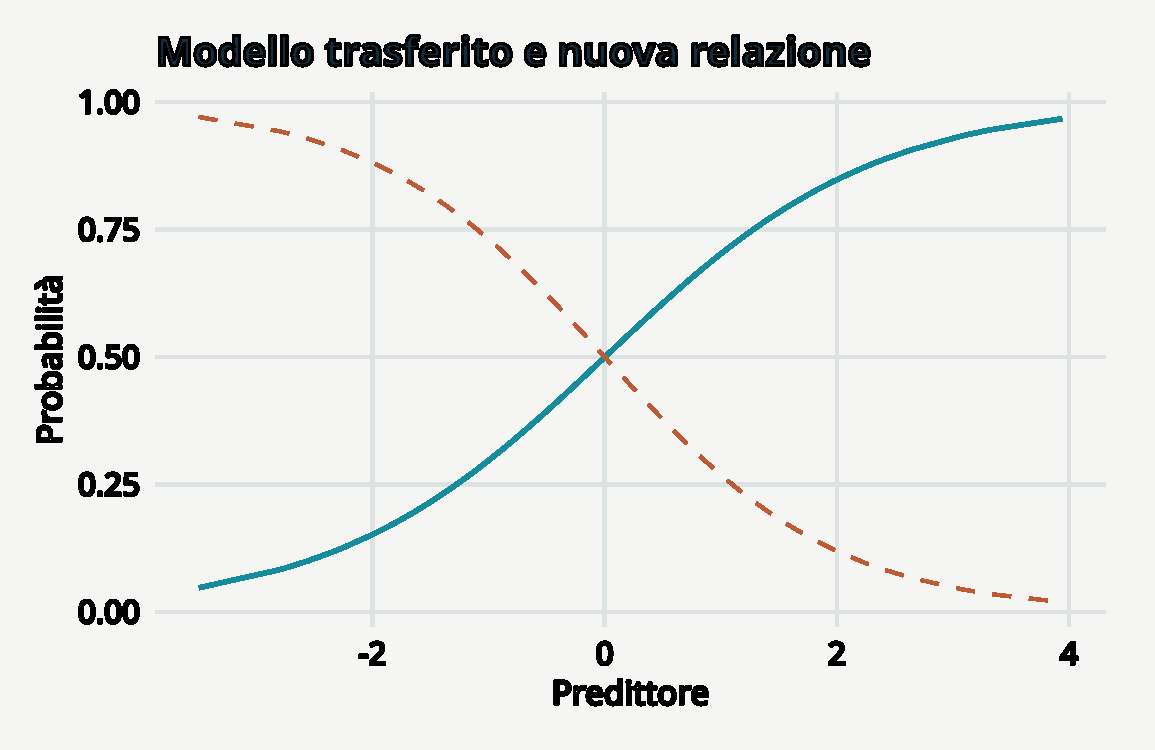
\includegraphics[width=\linewidth,height=5.6cm,keepaspectratio]{Esperimenti/m16-trasferimento-B.pdf}\par}
\PSmall{Pendenza nel nuovo territorio: 1 $\to$ -1. Tutti gli altri parametri e il seme sono fissi.}
}};
\node[anchor=north west,inner sep=0] at([xshift=10.85cm,yshift=-2.12cm]current page.north west){\Colonna{8.16cm}{\PLabel{Confronto fra gli scenari}
{\fontsize{10.2}{12.8}\selectfont\begin{tabular}{@{}>{\raggedright\arraybackslash}p{0.48\linewidth}@{\hspace{.13cm}}>{\raggedright\arraybackslash}p{0.224\linewidth}@{\hspace{.13cm}}>{\raggedright\arraybackslash}p{0.224\linewidth}@{}}\toprule Grandezza & A & B\\[2.3pt]
\midrule 
Accuratezza nuova popolazione & 0,67 & 0,33\\[2.3pt]
Brier nuova popolazione & 0,197 & 0,379\\[2.3pt]
Pendenza stimata nel training & 0,859 & 0,859\\[2.3pt]
\bottomrule\end{tabular}\par}
\vspace{.25cm}\PBody{Invertendo la pendenza nel nuovo territorio il modello trasferito conserva i coefficienti del training. L’accuratezza cala a 0,33 e il Brier score aumenta.}
}};
\node[anchor=north east,inner sep=0] at([xshift=17.1cm,yshift=-12.04cm]current page.north west){\fontsize{7.7}{9}\selectfont \href{https://marzione00.github.io/Lab_Geo/\#laboratorio/m16-trasferimento}{\color{Classical}\bfseries Apri il laboratorio · m16-trasferimento}};
\end{tikzpicture}\end{frame}

\begin{frame}[plain]\hypertarget{slide61}{}
\bookmark[level=1,page=61]{Dal risultato alla relazione}
\begin{tikzpicture}[remember picture,overlay]
\PilotChrome{Dal risultato alla relazione}{SINTESI}{61}{Descrivi unità di verifica, dominio di applicazione e possibili errori insieme alle prestazioni.}
\node[anchor=north west,inner sep=0] at([xshift=.96cm,yshift=-2.12cm]current page.north west){\Colonna{9.40cm}{\PLabel{Domanda di partenza}
\PBody{Quanto informa una classificazione corretta se la stazione del provino era già nel training?}
\PLabel{Risultato da discutere}
\PBody{Il centroide classifica correttamente i trenta provini del test sintetico. La separazione rispetta le stazioni e la regola costante di riferimento ottiene un terzo.}
}};
\node[anchor=north west,inner sep=0] at([xshift=10.85cm,yshift=-2.12cm]current page.north west){\Colonna{8.16cm}{\PLabel{Limiti della conclusione}
\PBody{Tre stazioni di test limitano ciò che si può concludere su un territorio nuovo. Un dataset sintetico molto separabile rende molti metodi ugualmente accurati.}
\vspace{.4cm}\href{https://marzione00.github.io/Lab_Geo/\#modulo-P11}{\color{Classical}\bfseries Prosegui · P11 · Classificare nuove stazioni sintetiche}}};
\end{tikzpicture}\end{frame}

\begin{frame}[plain]\hypertarget{slide62}{}
\bookmark[level=1,page=62]{Fonti, dati e codice per riprodurre le figure}
\begin{tikzpicture}[remember picture,overlay]
\PilotChrome{Fonti, dati e codice per riprodurre le figure}{RIFERIMENTI}{62}{Porta nel territorio nuovo la trasformazione stimata sul training e verifica le probabilità trasferite.}
\node[anchor=north west,inner sep=0] at([xshift=.96cm,yshift=-2.12cm]current page.north west){\Colonna{9.40cm}{\PLabel{Materiali del corso}
\PBody{Il fascicolo deriva dal modulo M16 di GeoStat Lab e dai materiali didattici di Marzio De Corato. I dati del caso guida sono didattici. Le simulazioni A e B riportano il proprio seme.}
\href{https://github.com/marzione00/Lab_Geo/blob/649f7cc577b96bd1044d81e78a2f530813e4f96b/moduli/M16/README.md}{\color{Classical}\bfseries Scheda e documentazione originale}\par\smallskip \href{https://github.com/marzione00/Lab_Geo/blob/649f7cc577b96bd1044d81e78a2f530813e4f96b/materiali/R/M16_figure.R}{\color{Classical}\bfseries Script R delle figure del corso}}};
\node[anchor=north west,inner sep=0] at([xshift=10.85cm,yshift=-2.12cm]current page.north west){\Colonna{8.16cm}{\PLabel{Nell’archivio dei sorgenti}
\PBody{Codice contiene i frammenti delle pagine. Esperimenti comprende i due programmi R e i risultati di ciascun confronto. Diagrammi contiene i disegni TikZ modificabili. Scena conserva il modello Blender della copertina.}
\vspace{.4cm}\href{https://marzione00.github.io/Lab_Geo/\#modulo-M16}{\color{Classical}\bfseries Apri Prisma su GeoStat Lab}}};
\end{tikzpicture}\end{frame}

\end{document}